%%%%%%%%%%%%%%%%%%%%%%%%%%%%%%%%%%%%%%%%
% datoteka diploma-vzorec.tex
%
% vzorčna datoteka za pisanje diplomskega dela v formatu LaTeX
% na UL Fakulteti za računalništvo in informatiko
%
% vkup spravil Gašper Fijavž, december 2010
% množica popravkov v januarju, februarju marcu 2011
% verzija 29. marec 2011

\documentclass[a4paper, 12pt]{book}

\usepackage[utf8x]{inputenc}   % omogoča uporabo slovenskih črk kodiranih v formatu UTF-8 
\usepackage[slovene,english]{babel}    % naloži, med drugim, slovenske delilne vzorce
\usepackage[pdftex]{graphicx}  % omogoča vlaganje slik različnih formatov 
\usepackage{fancyhdr}          % poskrbi, na primer, za glave strani
\usepackage{amssymb}           % dodatni simboli
\usepackage{amsmath}           % eqref, npr.
\usepackage{amsthm}
\usepackage{listings}
\usepackage{float}
\usepackage{algorithm}
\usepackage[noend]{algpseudocode}
\usepackage{listings}
\usepackage{color}
\usepackage{textcomp}
\usepackage{latexsym}
\usepackage{ifthen}
\usepackage[mathlines]{lineno}

%\newtheorem{theorem}{Theorem}
%\newtheorem{corollary}[theorem]{Corollary}
%\newtheorem{lemma}[theorem]{Lemma}
%\newtheorem{problem}[theorem]{Problem}
%\newtheorem{proposition}[theorem]{Proposition}
%\newtheorem{conjecture}[theorem]{Conjecture}

\renewcommand{\baselinestretch}{1.3} % ustrezen razmik med vrsticami

%oznake strani
\renewcommand{\chaptermark}[1]%
{\markboth{\MakeUppercase{\thechapter.\ #1}}{}} \renewcommand{\sectionmark}[1]%
{\markright{\MakeUppercase{\thesection.\ #1}}} \renewcommand{\headrulewidth}{0.5pt} \renewcommand{\footrulewidth}{0pt} 
\fancyhf{}
\fancyhead[LE,RO]{\sl \thepage} \fancyhead[LO]{\sl \rightmark} \fancyhead[RE]{\sl \leftmark}

\newcommand{\BibTeX}{{\sc Bib}\TeX}

\newcommand{\autfont}{\Large}
\newcommand{\titfont}{\LARGE\bf}
\newcommand{\D}{\ensuremath{\mathcal{D}}} 
\newcommand{\LL}{\ensuremath{\mathbb L}}
\newcommand{\RR}{\ensuremath{\mathbb R}}  % real numbers 
\newcommand{\NN}{\ensuremath{\mathbb N}}  % natural numbers 
\newcommand{\T}{\ensuremath{\mathcal{T}}} 
\newcommand{\OO}{\ensuremath{\mathcal{O}}} % big O notation
\newcommand{\clearemptydoublepage}{\newpage{\pagestyle{empty}\cleardoublepage}}
\setcounter{tocdepth}{1}	      % globina kazala

\def\length{\mathrm{len}}

% konstrukti
\newtheorem{izrek}{Izrek}[chapter]
%\newtheorem{trditev}{Trditev}[izrek]
\newtheorem{lema}[izrek]{Lema}
\newenvironment{dokaz}{\emph{Dokaz.}\ }{\hspace{\fill}{$\Box$}}

\definecolor{listinggray}{gray}{0.9}
\definecolor{lbcolor}{rgb}{0.9,0.9,0.9}
\definecolor{darkgreen}{rgb}{0.0, 0.2, 0.13}
\lstdefinestyle{customc}{
  belowcaptionskip=1\baselineskip,
  breaklines=true,
  frame=L,
  xleftmargin=\parindent,
  language=C,
  showstringspaces=false,
  basicstyle=\footnotesize\ttfamily,
  keywordstyle=\bfseries\color{red},
  commentstyle=\itshape\color{green},
  identifierstyle=\color{blue},
  stringstyle=\color{orange},
}

\lstset{escapechar=@,style=customc}
\lstset{
%backgroundcolor=\color{lbcolor},
    tabsize=4,    
%   rulecolor=,
    language=C++,
        basicstyle=\scriptsize,
        upquote=true,
        aboveskip={1.5\baselineskip},
        columns=fixed,
        showstringspaces=false,
        extendedchars=false,
        breaklines=true,
        prebreak = \raisebox{0ex}[0ex][0ex]{\ensuremath{\hookleftarrow}},
        frame=single,
        numbers=left,
        showtabs=false,
        showspaces=false,
        showstringspaces=false
%        \lstdefinestyle{C++}{language=C++,style=numbers}’.
}
\lstset{
    %backgroundcolor=\color{lbcolor},
    tabsize=4,
  language=C++,
  captionpos=b,
  tabsize=3,
  frame=lines,
  numbers=left,
  numberstyle=\tiny,
  numbersep=5pt,
  breaklines=true,
  showstringspaces=false
}

\begin{document}
\selectlanguage{slovene}
\frontmatter
\setcounter{tocdepth}{2}
\setcounter{page}{1} %
\renewcommand{\thepage}{}       % preprecimo težave s številkami strani v kazalu 

%%%%%%%%%%%%%%%%%%%%%%%%%%%%%%%%%%%%%%%%
%naslovnica
 \thispagestyle{empty}%
   \begin{center}
    {\large\sc Univerza v Ljubljani\\%
      Fakulteta za matematiko in fiziko\\
      Fakulteta za računalništvo in informatiko}%
    \vskip 10em%
    {\autfont Lazar Milinković\par}%
    {\titfont Implementacija algoritmov za probleme najkrajših poti v geometrijskih grafih \par}%
    {\vskip 2em \textsc{MAGISTRSKO DELO\\[2mm] 
    UNIVERZITETNI ŠTUDIJSKI PROGRAM DRUGE STOPNJE RAČUNALNIŠTVO IN MATEMATIKA}\par}%
    \vfill\null%
    {\large \textsc{Mentor}: dr. Sergio Cabello \par}%
    {\vskip 2em \large Ljubljana 2016 \par}%
\end{center}
% prazna stran
\clearemptydoublepage

%%%%%%%%%%%%%%%%%%%%%%%%%%%%%%%%%%%%%%%%
%copyright stran
\thispagestyle{empty}
\vspace*{8cm}
{\small \noindent
Rezultati diplomskega dela so intelektualna lastnina avtorja in Fakultete za ma\-te\-ma\-ti\-ko in fiziko Univerze v Ljubljani. 
Za objavljanje ali izkoriščanje rezultatov di\-plom\-ske\-ga dela je potrebno pisno soglasje avtorja, Fakultete za ma\-te\-ma\-ti\-ko in 
fiziko ter mentorja.}


\begin{center} 
\mbox{}\vfill
\emph{Besedilo je oblikovano z urejevalnikom besedil \LaTeX.} 
\end{center}
% prazna stran
\clearemptydoublepage

%%%%%%%%%%%%%%%%%%%%%%%%%%%%%%%%%%%%%%%%
% stran 3 med uvodnimi listi
\noindent
Namesto te strani {\bf vstavite} original izdane teme diplomskega 
dela s podpisom mentorja in dekana ter žigom fakultete, ki ga diplomant
dvigne v študent\-skem referatu,  preden odda izdelek v vezavo!

% prazna stran
\clearemptydoublepage

%%%%%%%%%%%%%%%%%%%%%%%%%%%%%%%%%%%%%%%%
% izjava o avtorstvu
\vspace*{1cm}
\begin{center} 
{\Large \textbf{\sc Izjava o avtorstvu magistrskega dela}}
\end{center}

\vspace{1cm}
\noindent Spodaj podpisani Lazar Milinković,
z vpisno številko \textbf{27122037}, sem avtor magistrskega dela z naslovom:
   
\vspace{0.5cm}
\emph{Implementacija algoritmov za probleme najkrajših poti v geometrijskih grafih}

\vspace{1.5cm}
\noindent S svojim podpisom zagotavljam, da:
\begin{itemize}
	\item sem magistrsko delo izdelal samostojno pod mentorstvom 
		dr.\ Sergia Cabella,

	\item	so elektronska oblika magistrskega dela, naslov (slov., angl.), povzetek (slov., angl.) ter ključne besede (slov., angl.) identični s tiskano obliko magistrskega dela
	\item soglašam z javno objavo elektronske oblike diplomskega dela v zbirki ''Dela FRI''.
\end{itemize}

\vspace{1cm}
\noindent V Ljubljani, dne 11. januarja 2016 \hfill Podpis avtorja:

% prazna stran
\clearemptydoublepage

%%%%%%%%%%%%%%%%%%%%%%%%%%%%%%%%%%%%%%%%
% zahvala
\thispagestyle{empty}\mbox{}\vfill\null\it%
 
\rm\normalfont

% prazna stran
\clearemptydoublepage


%%%%%%%%%%%%%%%%%%%%%%%%%%%%%%%%%%%%%%%%
% kazalo
\def\thepage{}% preprecimo tezave s stevilkami strani v kazalu 
\tableofcontents{}


% prazna stran
\clearemptydoublepage

%%%%%%%%%%%%%%%%%%%%%%%%%%%%%%%%%%%%%%%%
% povzetek 
\addcontentsline{toc}{chapter}{Povzetek}
\chapter*{Povzetek}
 

%%%%%%%%%%%%%%%%%%%%%%%%%%%%%%%%%%%%%%%%
% abstract
\selectlanguage{english}
\addcontentsline{toc}{chapter}{Abstract}
\chapter*{Abstract}


\selectlanguage{slovene}
% prazna stran
\clearemptydoublepage

%%%%%%%%%%%%%%%%%%%%%%%%%%%%%%%%%%%%%%%%
\mainmatter
\setcounter{page}{1}
\pagestyle{fancy}

\chapter{Uvod}
V poglavju 2 je na kratko opisana programska knjižnica CGAL. Osredotočili smo se na osrednje ideje, uporabljene pri jedru knjižnice, na katerem temeljijo vsi ostali deli paketa, ter tiste strukture, ki so bile uporabljene pri implementaciji našega algoritma. V poglavju 3 je predstavljen teoretični del algoritma. Podrobno so opisane vse podatkovne strukture, celotni potek algoritma ter njegova časovna in prostorska kompleksnost. V poglavju 4 je predstavljena implementacija algoritma. Ponovno so opisane vse uporabljene podatkovne strukture in nekatere spremembe v header datotekah CGAL-a z razredi, ki predstavljajo te strukture. Podrobno so opisani tudi deli algoritma, kjer se pojavijo razlike med teoretičnim opisom in implementacijo. V poglavju 5 so predstavljeni rezultati; prikazani so časi izvajanja in prostorska poraba celotnega algoritma za različno število vhodnih točk. Enako smo storili posebej za nekatere podatkovne strukture, npr. Kd drevesa, Voronoijev diagram in SSSP drevesa.

\clearemptydoublepage


\chapter{CGAL in uporabljene matematične strukture}
\label{ch1}

V tem poglavju so na kratko opisani programska knjižnica CGAL in podatkovne strukture, uporabljene v naših algoritmih. Za bolj podroben opis glej (citiraj van kreveld, cgal.org in nekaj za bfs, sssp in grid graf). Vse podatkovne strukture so opisane za dvodimenzionalni primer.
\section{CGAL}
CGAL (Computational Geometry Algorithms Library) je programski paket, ki omogoča enostaven dostop do učinkovitih in zanesljivih geometrijskih algoritmov v obliki C++ knjižnice. Uporablja se na različnih področjih, ki potrebujejo geometrijsko računanje, kot so geografski informacijski sistemi, računalniško podprto načrtovanje, molekularna biologija, medicina, računalniška grafika in robotika. Knjižnica vsebuje:

\begin{itemize}
\item jedro z geometrijskimi osnovami, kot so točke, vektorji, črte, predikati za preizkušanje stvari (na primer relativni položaji točk) in opravila, kot so izračunavanje presekov ter razdalj
\item osnovno knjižnico, ki je zbirka standardnih podatkovnih struktur in geometrijskih algoritmov, kot so konveksna ovojnica v 2D/3D, Delaunayova triangulacija v 2D/3D, ravninski zemljevid, polieder, Voronoijev diagram, območna drevesa (range trees) itd.
\item podporna knjižnica, ki ponuja vmesnike do drugih paketov, na primer za V/I in vizualizacijo. 
\end{itemize}

Ker cilj magistrske naloge ni bila implementacija osnovnih geometrijskih struktur, ki sicer predstavljajo pomembno osnovo našega algoritma, smo se odločili uporabiti omenjeno knjižnico in si s tem prihraniti čas in odvečno delo. Posledično je seveda celoten algoritem implementiran v jeziku C++.

Pri nekaterih razredih knjižnice smo morali spremeniti kodo ali dodati kaj novega. Podrobnosti so razložene v nadaljevanju opisa implementacije pri ustreznih delih algoritma.

??? 
natancnost: cartesian, kaj pa leda, homogenous?
povej kaj o traits, templated strukturami ($Point_2$) 

\section{BFS drevesa}
\section{SSSP drevesa}
Drevo najkrajših poti z eno izvorno točko je vpeto drevo $T$ grafa $G$ s korenom $v$, za katerega velja, da je razdalja poti od $v$ do $u \in T$ enaka razdalji najkrajše poti od $v$ do $u$. Tako drevo lahko zgradimo s pomočjo algoritma za iskanje najkrajše poti med dvema danima točkama (tipična primera sta Dijsktrov in Bellman-Fordov algoritem). Izvorno točko $v$ fiksiramo in poženemo algoritem za vse pare $(v, u), v,u \in G.$ Časovna kompleksnost Dijkstrovega algoritma je $\OO((m+n)\log n)$, kjer je $n$ število vozlišč, $m$ pa število povezav v $G$. Ker moramo algoritem pognati za $n-1$ parov, lahko drevo zgradimo v času $\OO((n^2 + nm)\log n)$. Če predpostavimo, da za vhodni graf $G$ veljajo določene omejitve (v primeru našega algoritma povezava med vozliščema v grafu obstaja samo, če je njuna razdalja največ 1), ki se jih da izkoristiti pri izgradnji hitrejšega algoritma, se časovna kompleksnost lahko izboljša.
\section{Graf kvadratne mreže}
$https://en.wikipedia.org/wiki/Lattice_graph_Square_grid_graph$
\begin{figure}
\centerline{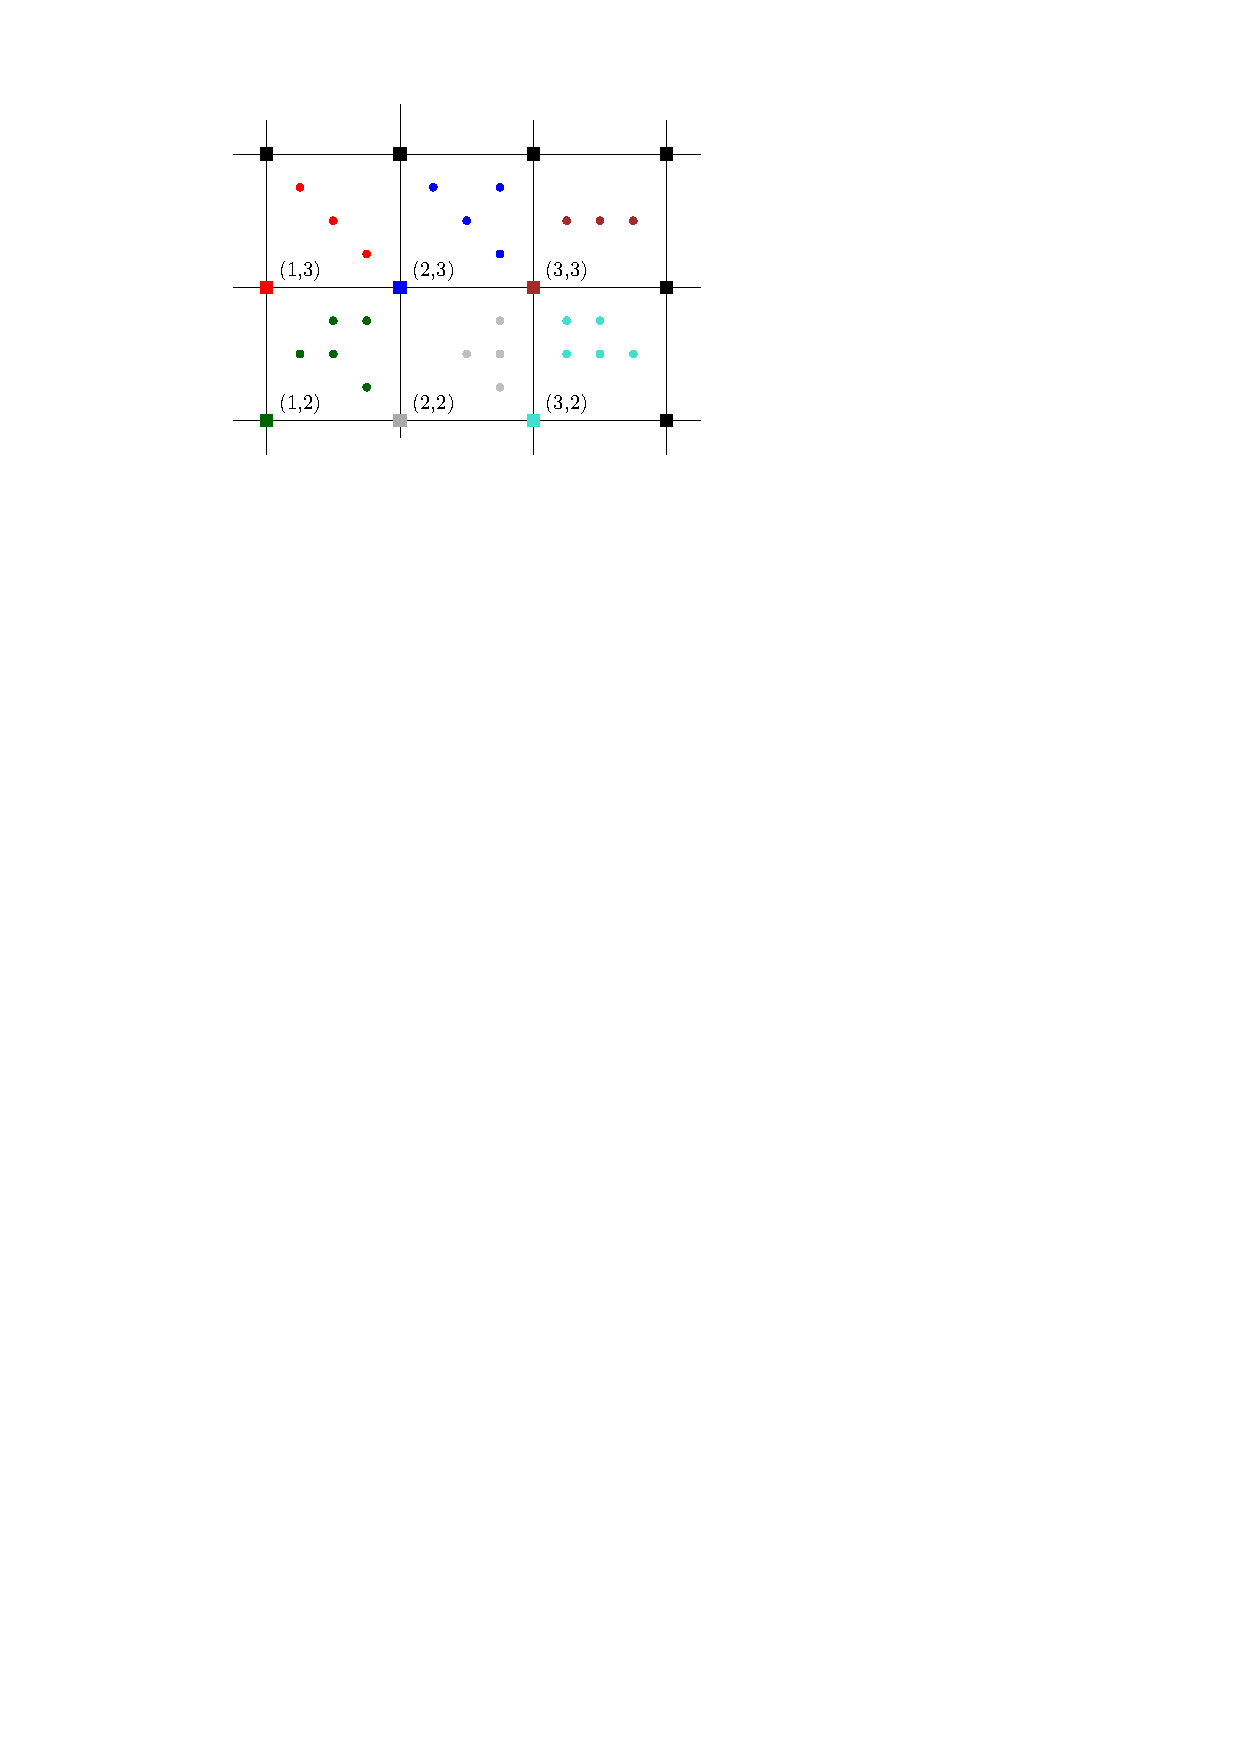
\includegraphics[scale=1.2]{pics/grid.pdf}}
\caption{Evklidski Voronoijev diagram brez degeneracij, označen z rdečimi odebeljenimi povezavami. Voronoijeva središča, obarvana z modro barvo, predstavljajo hkrati tudi vozlišča v Delaunayevi triangulaciji, dualni Voronoijevemu diagramu, in je označena s tanjšimi črnimi povezavami.}
\label{grid}
\end{figure}


\section{Delaunayeva triangulacija}
\subsection{Implementacija v CGAL}


\section{Voronoijev diagram}
\begin{figure}
\centerline{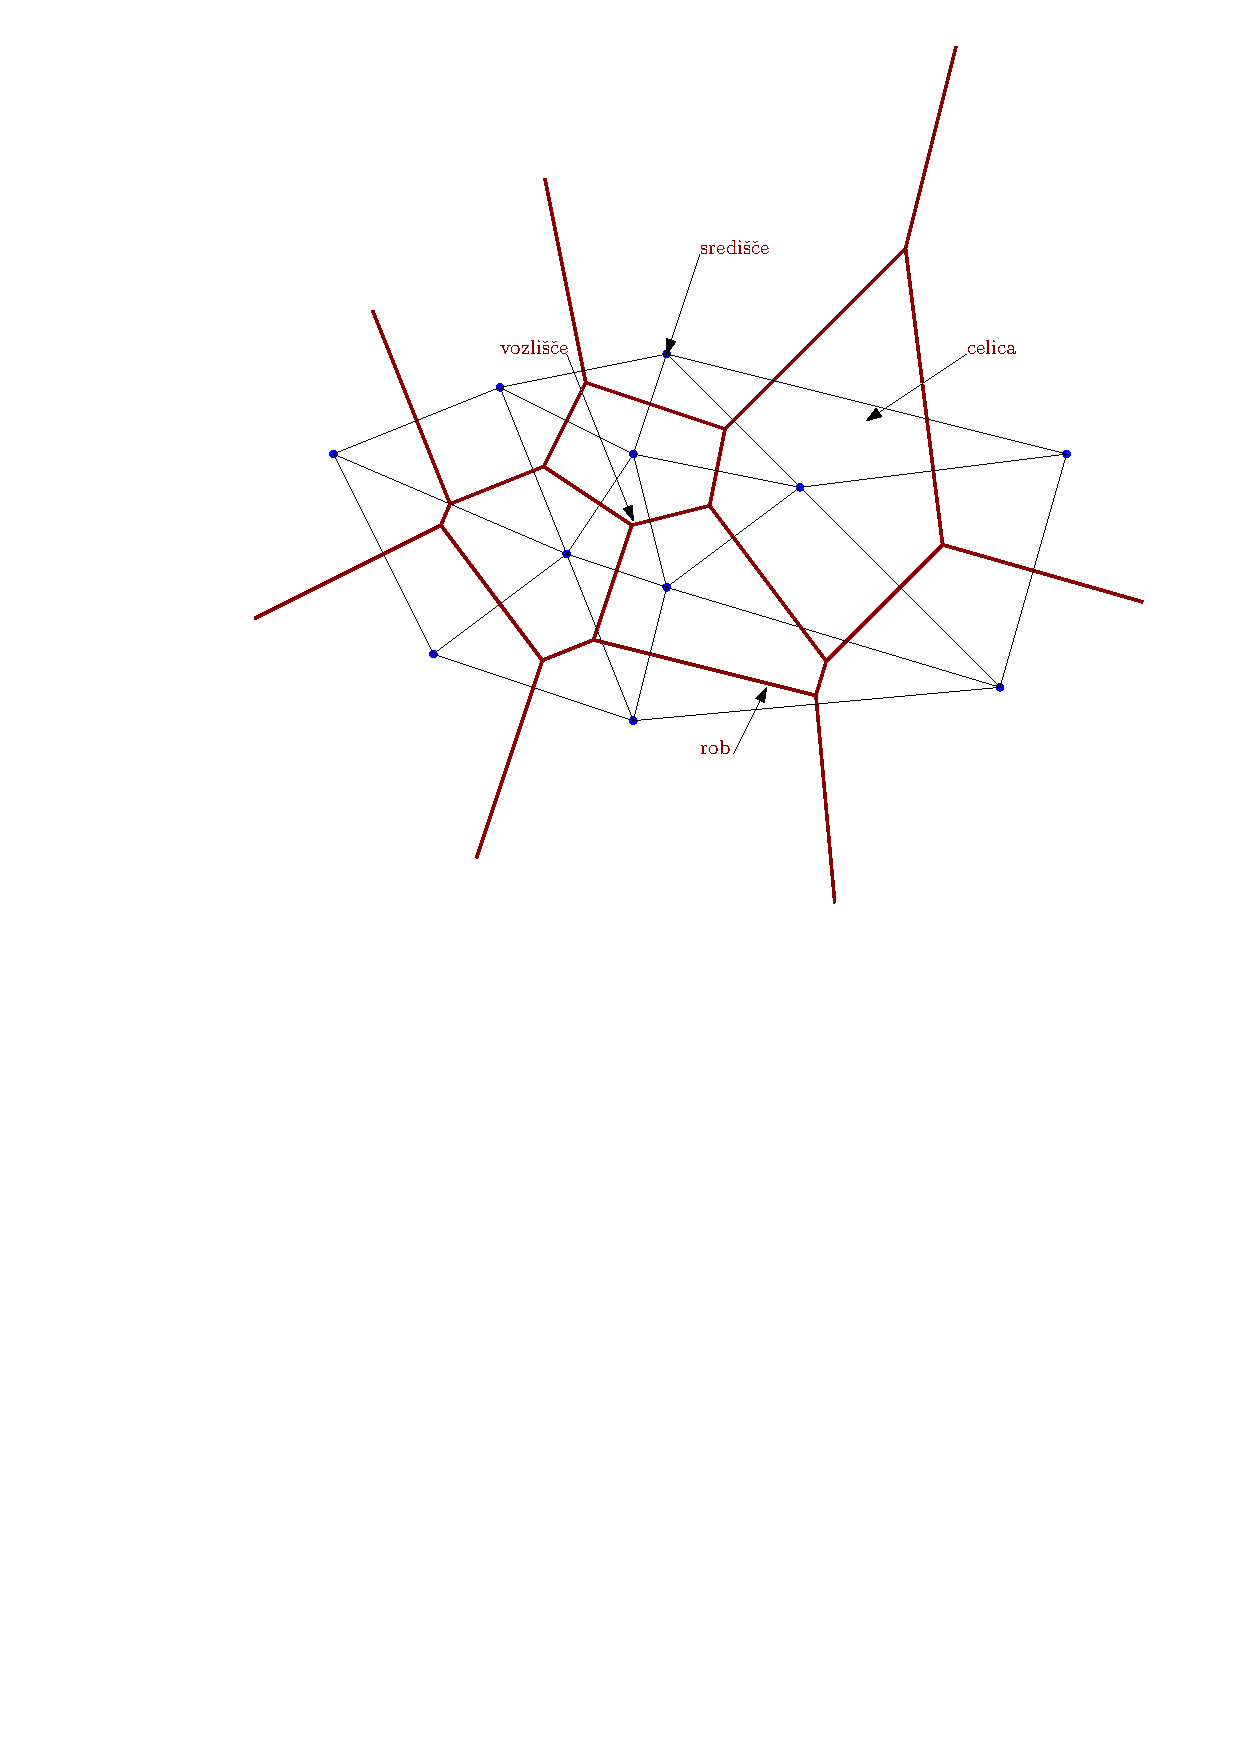
\includegraphics[scale=1.2]{pics/voronoi-dt.pdf}}
\caption{Evklidski Voronoijev diagram brez degeneracij, označen z rdečimi odebeljenimi povezavami. Voronoijeva središča, obarvana z modro barvo, predstavljajo hkrati tudi vozlišča v Delaunayevi triangulaciji, dualni Voronoijevemu diagramu, in je označena s tanjšimi črnimi povezavami.}
\label{vd}
\end{figure}

Voronoijev diagram ~\cite{cgalVor} je definiran na množici točk, imenovanih Voronoijeva središča (angleško $sites$), ki ležijo v nekem prostoru $\sum$, in z metriko oziroma funkcijo razdalje med točkami. Za ravninski Voronoijev diagram, opisan v nadaljevanju, velja $\sum = \mathbb{R}^2$.

Naj bo S = $S = \{S_1,S_2,...,S_n\}$ množica Voroijevih središč in naj bo $\delta(x,S_i)$ funkcija razdalje med središčem $S_i$ in neko točko $x \in \mathbb{R}^2$. Množica točk $V_{ij}$, ki so bližje središču $S_i$ kot središču $S_2$ na podlagi funkcije $\delta(x,\cdot)$, je množica:

\begin{equation}
V_{ij} = \{x \in \mathbb{R}^2: \delta(x,S_i) < \delta(x,S_j)\}. 
\end{equation}

Množico $V_i$ točk, ki so bližje središču $S_i$ kot kateremu koli drugemu središču, lahko potem definiramo kot množico:

\begin{equation}
V_i = \bigcap_{i \neq j} V_{ij} .
\end{equation}



Množico $V_i$ imenujemo tudi Voronoijeva celica ali Voronijevo lice središča $S_i$. Lokus točk, ki so enako oddaljene od dveh središč, se imenuje Voronijev bisektor. Povezani podmnožici slednjega pravimo Voronoijev rob. Točki, ki je enako oddaljena od treh ali več središč, pravimo Voronoijevo vozlišče. Voronoijev diagram na množici $S$ in z metriko $\delta(x,\cdot)$ je zbirka Voronoijevih celic, robov in vozlišč ter je primer ravninskega grafa.

Celice si ponavadi predstavljamo kot 2-dimenzionalne, robove kot 1-dimenzionalne in vozlišča kot 0-dimenzionalne objekte. Za določene kombinacije središč in metrik to ne drži. Voronijev diagram z metriko $L_1$ ali $L_{\infty}$ lahko na primer vsebuje dvodimenzionalne robove. Takim Voronoijevim diagramom, za katere zgornja omejitev drži in imajo lastnost, da so njihove celice preprosto povezano območje v ravnini, pravimo preprosti Voronoijevi diagrami. Najbolj tipičen primer slednjih je evklidski Voronoijev diagram (slika ~\ref{vd}), ki ga uporabljamo v napem algoritmu.

\subsection{Voronoijev diagram v CGAL}
Knjižnica CGAL ponuja razred Voronoi\texttt{\_}diagram\texttt{\_}2$<DG,AT,AP>$, ki deluje kot prilagoditveni paket. Ta Delaunayevo triangulacijo na podlagi podanih kriterijev prilagodi pripadajočemu Voronoijevemu diagramu, ki je predstavljen kot DCEL (doubly connected edge list) struktura. Paket je torej zasnovan tako, da na zunaj deluje kot DCEL struktura, znotraj pa v resnici hrani strukturo grafa, ki predstavlja graf triangulacije.

Razred je parametriziran s tremi predlogami. Prvi, DT, mora biti primerek, ki predstavlja koncept razreda DelaunayGraph\texttt{\_}2. Primeri takih struktur so Delaunayeva triangulacija, navadna triangulacija in Apollonov graf. Druga predloga, AT, predstavlja lastnosti prilagoditve ter definira tipe struktur in funktorje, ki jih razred potrebuje za dostop do geometrijskih lastnosti Delaunayeve triangulacije. Funktor mora biti recimo definiran za konstrukcijo Voronoijevih vozlišč iz njihovih dualnih lic v Delaunayevi triangulaciji. Za našo implementacijo algoritma ločevanja z diski je pomemben funktor za poizvedbe najbližjih središč, ki kot rezultat vrne informacijo o tem, koliko in katera središča so enako oddaljena od točke poizvedbe. Bolj konkretno, rezultat je Delaunayevo vozlišče, lice ali rob, na katerem točka poizvedbe leži oziroma z njim sovpada. Če je na primer točka poizvedbe $q$, enako oddaljena od treh središč, potem sovpada z nekim Voronoijevim vozliščem, zato funktor vrne Delaunayevo lice, ki je dualno temu vozlišču. Razred, ki predstavlja Delaunayevo lice, omogoča iteracijo po Delaunayevih vozliščih, ki definirajo lice, ta pa so dualna trem Voronoijevim središčem.

Tretja predloga predstavlja režim adaptacije Delaunayeve triangulacije Voronoijevemu diagramu. 
Če množica središč, ki določa graf Delaunayeve triangulacije, vsebuje podmmnožice središč, ki so v degeneriranem položaju, potem ima dualni graf - Voronoijev diagram - lahko robove dolžine nič in po možnosti tudi celice s ploščino nič. Režim adaptacije določa, kaj storiti v takih primerih. V našem projektu smo uporabili tip režima, imenovan $Delaunay\texttt{\_}triangulation\texttt{\_}caching\texttt{\_}degeneracy\texttt{\_}removal\texttt{\_}policy\texttt{\_}2$. Kot pove že ime, ta tip poskrbi, da so vse zgoraj opisane celice in robovi odstranjeni iz Voronoijevega diagrama. Poleg tega uporablja $cache$ pri ugotavljanju, ali ima določena celica oziroma rob degenerirane lastnosti. Ker je slednje precej zahtevna operacija, se ta tip izplača pri vhodnih podatkih (središčih) z veliko degeneriranimi primeri.
 

\section{Območna drevesa}
Območna drevesa so še ena podatkovna struktura za poizvedbe nad pravokotnimi območji. V primerjavi s kd drevesi imajo boljši čas poizvedbe ($\OO(\log^2 n)$), ampak slabšo prostorsko kompleksnost ($\OO(n\log n)$).

\begin{figure}
\centerline{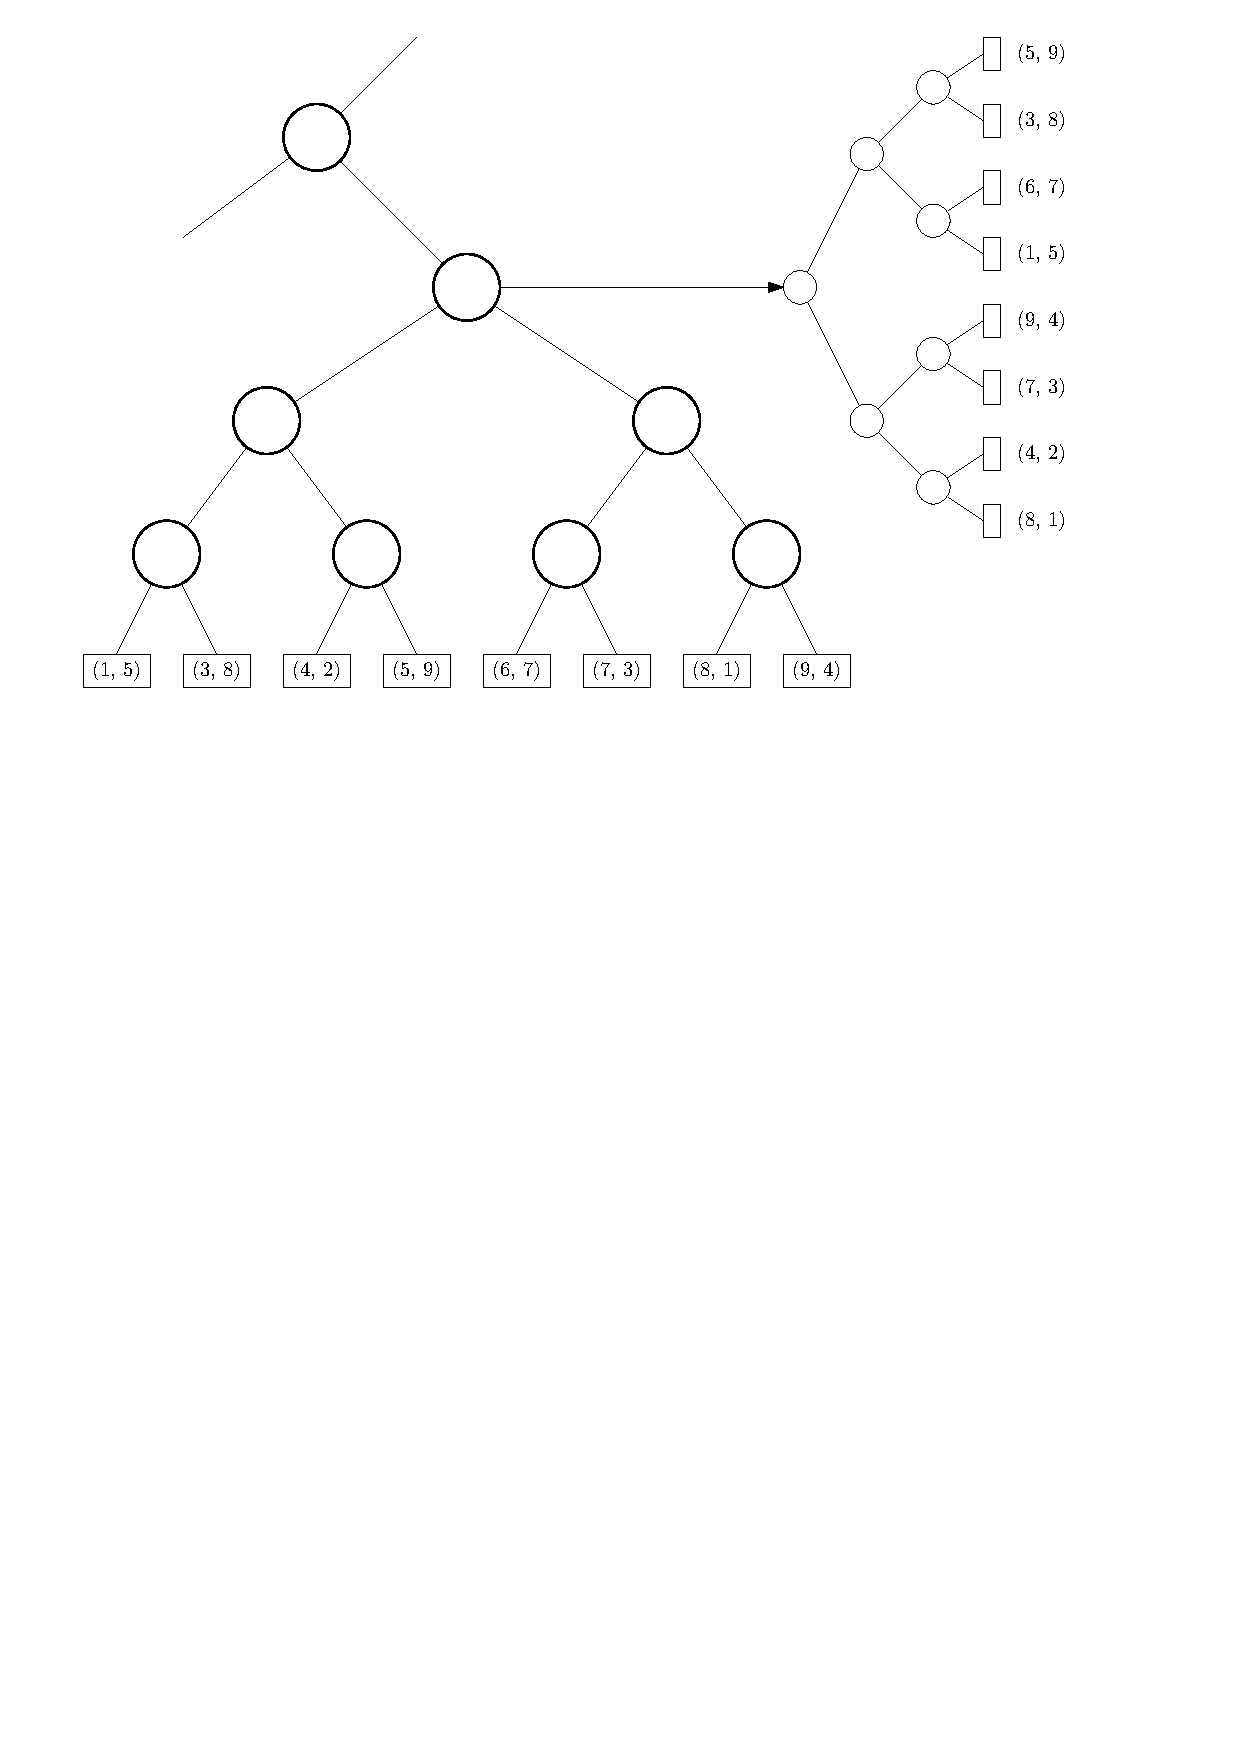
\includegraphics[scale=1.2]{pics/rangeTree.pdf}}
\caption{Dvodimenzionalno območno drevo.}
\label{range-primer}
\end{figure}


\chapter{Teorija}
\section{Predstavitev problema}
Naj bo $\D$ množica skladnih enotskih krogov na Evklidski ravnini, ki jih definirajo njihove središčne točke.  $z$ in $z'$ naj bosta dve dani točki, ki nista vsebovani v nobenem krogu. Za $\D$ rečemo, da ločuje $z$ in $z'$, če vsaka pot v ravnini od $z$ do $z'$ seka nek krog v $\D$.

Problem iskanja minimalne kardinalne podmnožice $\D$, ki ločuje $z$ in $z'$, lahko formalno zapišemo kot:

\begin{align*}
	\min ~~		& |\D'|\\
	 \mbox{tako da}~~ & \D'\subset \D\\
				&	\D'\text{ ločuje $z$ in $z'$}. 
\end{align*}

\begin{figure}
\centerline{\includegraphics[scale=0.6,page=4]{pics/unitdisks.pdf}}
\caption{Slikovna predstavitev problema. Točki $s$ in $t$ ločuje množica krogov, definiranih z njihovimi središčnimi točkami.}
\label{separation}
\end{figure}

Cilj našega algoritma za ločevanje enotskih krogov je rešiti ta problem v skoraj kvadratičnem času. Do take časovne kompleksnosti pridemo tudi s pomočjo še enega našega algoritma za izgradnjo drevesa najkrajših poti iz enega, danega izhodišča. Oba algoritma sta opisana v nadaljevanju, prav tako dokaza za njuno časovno kompleksnost.

Naj bo $P$ množica točk, ki predstavljajo središča krogov $\D$. $P$ predstavlja vhod našega algoritma in vse operacije ter uporabljene podatkovne strukture se vrtijo okoli te množice. Kardinalnost množice je enaka $n$.

\begin{figure}
\centerline{\includegraphics[scale=0.6,page=5]{pics/unitdisks.pdf}}
\caption{Graf $G(P)$, zgrajen nad množico $P$ v sliki ~\ref{separation}.}
\label{gdisks}
\end{figure}

Naj bo $G(P)$ graf z množico vozlišč $P$ s povezavo med točkama $p,q \in P$, če velja $|pq| <= 1$ z evklidsko metriko. Vse povezave so neobtežene.

\begin{figure}
\centerline{\includegraphics[scale=0.6,page=3]{pics/separation.pdf}}
\caption{Minimalna podmnožica točk iz slike ~\ref{separation}, ki ločuje $s$ in $t$, med seboj povezanih z modrimi povezavami. Podmnožica je vedno zaprta pot.}
\label{walk}
\end{figure}

V nadaljevanju bomo namesto $G(P)$ pisali preprosto $G$, brez izgube splošnosti pa predpostavili, da je $z=(0,0)$ in $z'=(0,s)$. $zz'$ je torej daljica, v nadaljevanju imenovana $\sigma$, ki je vsebovana v koordinatni osi $y$. Če dana vhodna daljica ne leži na osi $y$, lahko naredimo translacijo nad $\sigma$ in $P$; če poleg tega tudi vertikalna ni, naredimo še rotacijo (kjer pa lahko pride do numeričnih napak). 
\section{SSSP drevo}

V tem poglavju je opisan algoritem za drevo SSSP (ang. single source shortest path). Gre za preiskovanje v širino nad grafom $G(P)$ brez dejanske izgradnje grafa. Vhod algoritma je torej $P$, pri izgradnji drevesa pa se uporablja abstrakten graf G(P).

\begin{figure}
\centerline{\includegraphics[scale=0.6,page=6]{pics/unitdisks.pdf}}
\caption{Drevo najbližjega soseda, ki hrani 6 točk, predstavljeno v obliki seznama. Za vsako celico so prikazani indeksi točk, ki jih hrani objekt v njej.}
\label{nnarray}
\end{figure}

Algoritem dobi kot vhod poleg množice $P$ izvorno točko $s\in P$ in nato inkrementalno v vsaki iteraciji dodaja točke h grafu. Množico točk, dodanih k drevesu v $i$-ti iteraciji, označimo kot
\[	W_i = \{ p\in P \mid d_{G(P)}(s,p) = i\}.
	\]

Velja torej $W_0 = \{s\}$. Za izgradnjo $W_i$ ne potrebujemo celotnega grafa, zgrajenega do $i-1$-te iteracije, temveč samo množico $W_{i-1}$.  Za vsak $q\in W_i$ velja, da je povezan s točko $p = NN(q, W_{i-1})$. $p$ je torej izmed točk v $W_{i-1}$ najbližje $q$.

Pri izgradnji $W_i$ ne pregledujemo vseh še ne dodanih točk. Že v samem začetku najprej zgradimo Delaunayevo triangulacijo $DT(P)$, ki nam je v pomoč pri iskanju primernih kandidatov za $W_i$. To so:

\begin{itemize}
\item točke sosednje $W_{i-1}$ v $DT(P)$
\item točke sosednje (do tega trenutka zgrajeni) $W_i$ v $DT(P)$.
\end{itemize} 

\begin{lema}
\label{lema1}
Naj bo $p$ točka v $P\backslash \{s\}$, za katero velja $d(s,p) < \infty$. Obstajata točka $w$ v $P$ in pot $\Pi$ v $DT(P)$ od $w$ do $p$, za kateri velja $d(s,w)+1 = d(s,p)$ in $d(s,p_j) = d(s,p)$ za vsako notranje vozlišče $p_j$ v $\Pi$.
\end{lema}

\begin{figure}
\centerline{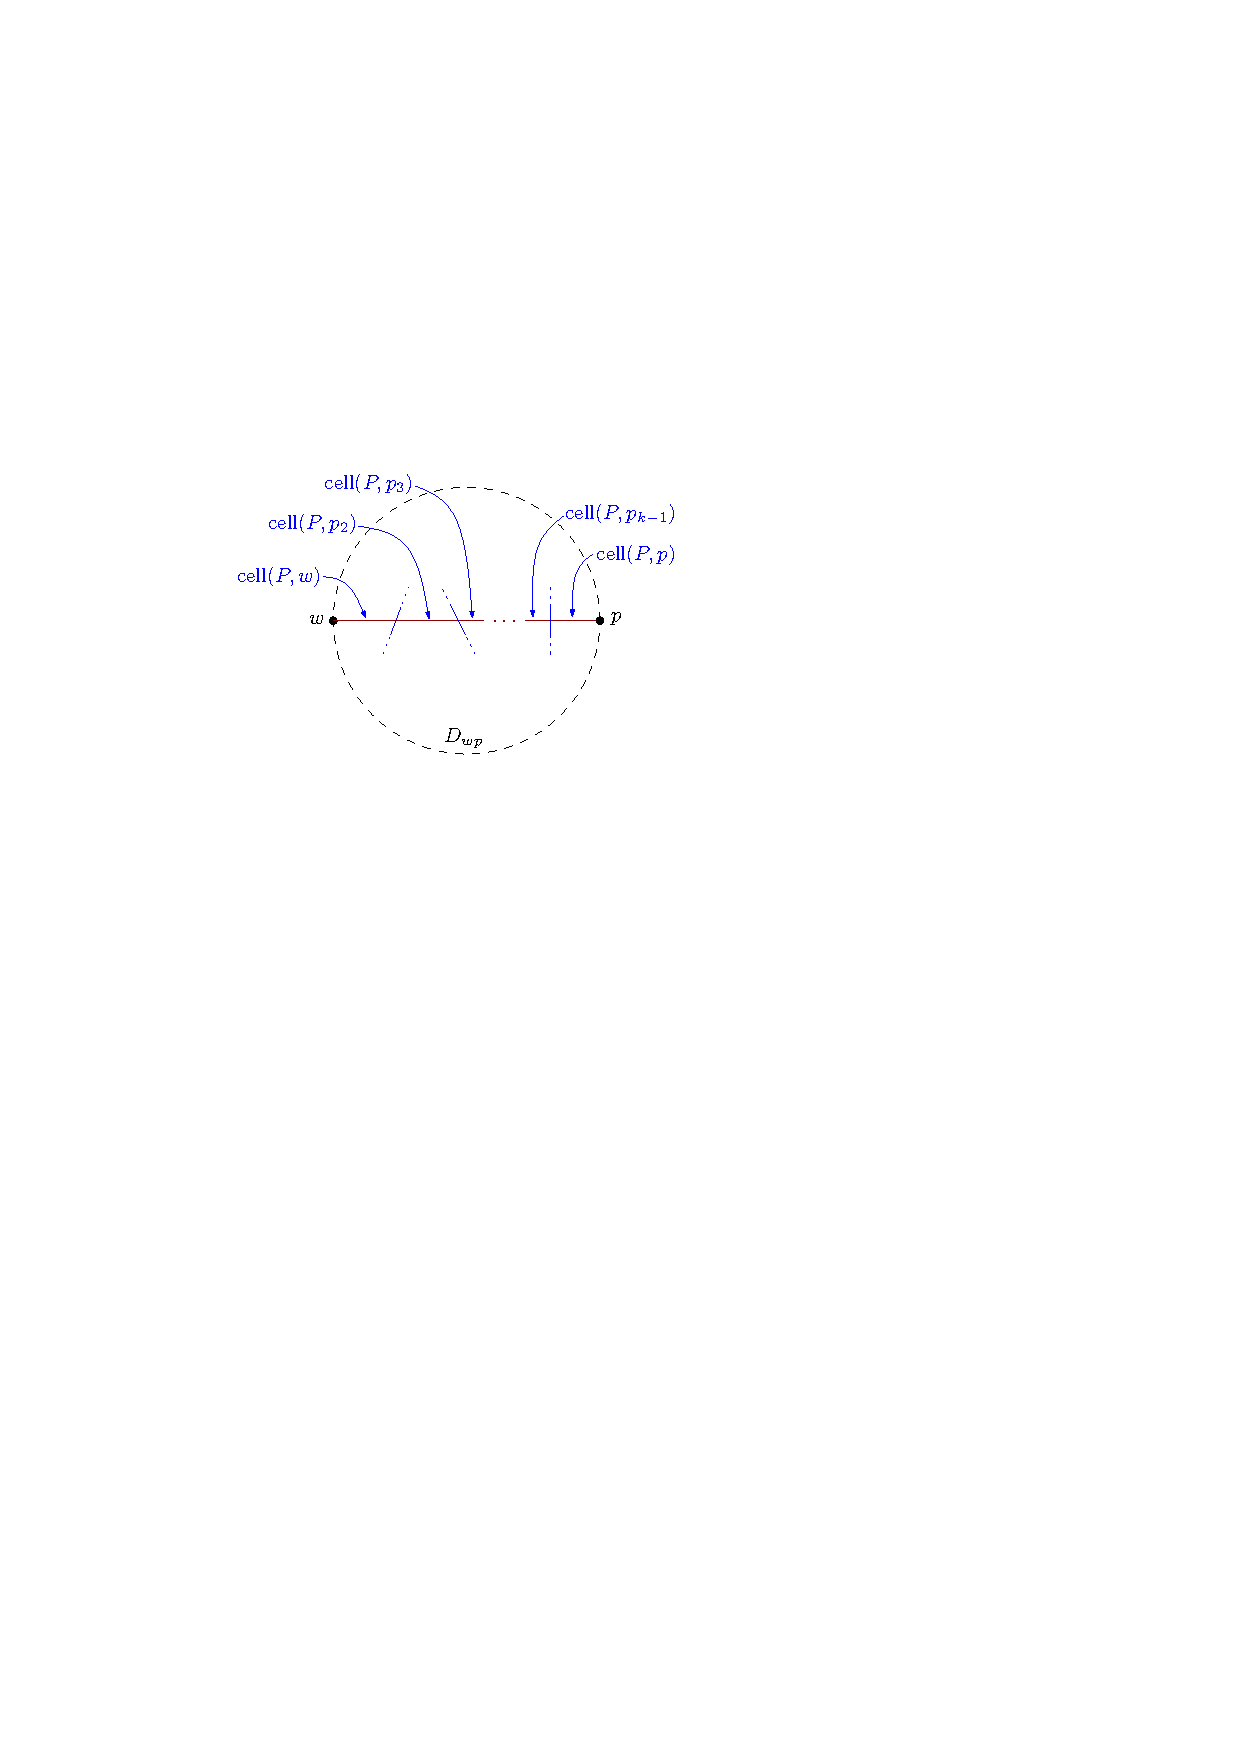
\includegraphics[scale=1]{pics/path.pdf}}
\caption{aa}
\label{c1c2}
\end{figure}

\begin{proof}
Naj bo $i = d(s,p)$, $w$ pa naj bo točka z $d(s,w) = i - 1$, ki je najbližje $p$ po evklidski razdalji. Ker $d(s,p) < \infty$, mora veljati $\|w - p\| \leq 1$. Naj bo $D_{wp}$ krog s premerom $wp$.

Predpostavimo, da segment $wp$ ne gre skozi nobeno vozlišče VD nad $P$.  Pobliže si poglejmo zaporedje Voronoijevih celic $cell(p_1, P),..., cell(p_k, P)$, ki ga seka segment $wp$, ko se sprehodimo od $w$ do $p$. Očitno velja $w = p_1$ in $p = p_k$. Za vsak $1 \leq j < k$ je povezava $p_jp_{j+1}$ v $DT(P)$, ker sta si celici $cell(p_j, P)$ in $cell(p_{j+1}, P)$ sosedni prek neke točke v $wp$. Pot $\pi = p_1p_2...p_k$ je zato vsebovana v $DT(P)$ in povezuje $w$ s $p$. Za katerikoli indeks $j$, kjer $1 < j < k$, naj bo $a_j$ katerakoli točka v $wp \cap cell(p_j, P)$. Ker velja $\|a_jp_j\| \leq \{\|a_jw\|, \|a_jp\|\}$, je točka $p_j$ vsebovana v $D_{wp}$. Potem je celotna pot $\pi$ vsebovana v $D_{wp}$, in ker je premer $D_{wp}$ največ 1, je vsaka povezava poti $\pi$ tudi v $G(P)$. S tem sklenemo, da je $\pi$ pot v $DT(P) \cap G(P)$.

Vzemimo katerokoli točko $p_j$ v $\pi$, ki je potem vsebovana v $D_{wp}$. Ker $\|w - p_j\| \leq \|w - p\| \leq 1$, velja $d(s, p_j) \leq d(s, w) + 1 = i$. Ker $\|p_j - p\| \leq \|w - p\| \leq 1$, velja $d(s, p_j) \geq d(s, p) - 1 = i - 1$. Ampak izbira $w$ kot točke najbližje $p$ pomeni, da $d(s, p_j) \neq i - 1$, ker $\|p_j - p\| < \|w - p\|$. Zato velja $d(s, p_j) = i$. Iz tega sklenemo, da za vsa notranja vozlišča $p_j$ v $\pi$ velja $d(s, p_j) = i$. 
\end{proof}

\begin{lema}
\label{lema2}
Na koncu algoritma $UnweightedShortestPath(P, s)$ velja:

\begin{equation}
\forall i \in \NN \cup \{0\}:  W_i = \{p\in P \mid d(s, p) = i\}.
\end{equation}

Poleg tega za vsako točko $p \in P \backslash \{s\}$ velja $dist[p] = d(s,p)$ in če velja $d(s,p) < \infty$, potem obstaja najkrajša pot v $G(P)$ od $s$ do $p$, v kateri je zadnja povezava $\pi [p]p$.
\end{lema}

\begin{proof}
Za dokaz uporabimo indukcijo nad $i$. $W_0 = \{s\}$ je nastavljen v vrstici 6 in kasneje ne spremeni vrednosti. Za $i = 0$ potem izjava velja.

Preden obravnavamo indukcijski korak, izpostavimo, da so množice $W_0, W_1,...$ parno disjunktne. To je razvidno tudi iz psevdokode. Točka $p$  je v vrstici 21 dodana v nek $W_i$, po tem, ko nastavimo $dist[p] = i$ v vrstici 18. Po tem je pogoj v vrstici 17 vedno neresničen in $p$ ni dodan v nobeno drugo množico $W_j$.

Vzemimo katerikoli $i \ge 0$. Po indukcijski predpostavki velja

\begin{equation}
W_{i-1} = \{p \in P \mid d(s,p) = i - 1\}.
\end{equation}

V algoritmu dodamo točke v $W_i$ samo v vrstici 21. Če je $p$ dodan v $W_i$, potem velja $\|p - w\| \leq 1$ za nek $w \in W_{i-1}$ zaradi pogoja v vrstici 17. Potem vsak $p$, dodan v $W_i$, zadostuje pogoju $d(s,p) \leq i$. Ker $p \notin W_{i-1}$, iz disjunkcije množic $W_0, W_1,...$ sledi $d(s,p) = i$. Sklenemo, da

\begin{equation}
W_i \subseteq \{p \in P \mid d(s,p) = i\}.
\end{equation}

Da dobimo vsebovanost v drugo smer, naj bo $p$ neka točka, za katero velja $d(s,p) = i$. Pokazati moramo, da je z algoritmom $p$ dodan v $W_i$. Vzemimo točko $w$ in pot $\pi = p_1...p_k$, zagotovljeno z lemo ~\ref{lema1}. Z indukcijsko hipotezo imamo $w = p_1 \in W_{i-1}$ in zato je $w$ dodan v $Q$ v vrstici 10. V nekem trenutku je povezava $p_1p_2$ obravnavana v vrstici 15 in točka $p2$ je dodana v $W_i$ in $Q$. Po $indukcijski tezi$(!!!) so potem vse točke $p_3,...,p_k$ dodane v $W_i$ in $Q$ (po možnosti v različnem vrstnem redu). Sledi, da je $p_k = p$ dodan v $W_i$ in zato

\begin{equation}
W_i = \{p \in P \mid d(s,p) = i \}.
\end{equation}

Ker je $p$ dodan v $W_i$ ob istem času, ko je nastavljen $dist[p] = i$, sledi, da $dist[p] = i = d(s,p)$. Ker $\pi[p] \in W_{i-1}$ in $\|p - \pi[p] \| \leq 1$ (vrstice 16, 17 in 19), obstaja najkrajša pot v $G(P)$ od $s$ do $p$, ki uporablja $(i-1)$-to povezavo poti od $s$ do $\pi[p]$, po indukciji pa ji sledi povezava $\pi[p]p$.
\end{proof}

Da dobimo odgovor na vprašanje, ali je nek kandidat $p\in W_i$, uporabimo podatkovno strukturo, ki zna v zglednem času najti najbližjega soseda $q$ in preveriti, če je razdalja med njima manjša ali enaka 1.

Celotna psevdokoda algoritma za izgradnjo drevesa je opisana spodaj.

\makeatletter
\def\BState{\State\hskip-\ALG@thistlm}
\makeatother

\begin{algorithm}
\caption{Algoritem za izgradnjo SSSP drevesa}\label{euclid}
\begin{algorithmic}[1]
\Procedure{buildTree}{}
\For {p $\in$ P}
\State dist$[p] \gets \infty$
\EndFor
\State dist$[r] \gets$ 0
\State zgradi Delaunayevo triangulacijo $DT(P)$
\State $W_{0} \gets \{ s \}$
\State $i \gets$ 1
\While {$W_{i-1} \neq \emptyset $}
\State zgradi pod. strukturo za poizvedbe najbližjega soseda v $W_{i-1}$
\State $Q \gets W_{i-1}$ ($\star$ generator točk kandidatk $\star$)
\State $W_{i} \gets \emptyset$
\While {$Q \neq \emptyset$}
\State $q$ naj bo poljubna točka v $Q$
\State odstrani $q$ iz $Q$
\For {povezava $qp$ v $DT(P)$}
\State $w \gets$ NN($W_{i-1},p$)
\If {dist$[p] = \infty$ and $|pw| \leq$ 1}
\State dist$[p] \gets i$
\State $\pi[p] \gets w$
\State dodaj $p$ v $Q$
\State dodaj $p$ v $W_{i}$
\EndIf
\EndFor
\EndWhile
\State $i \gets i + 1$
\EndWhile
\State \Return dist$[\cdot]$
\EndProcedure
\end{algorithmic}
\end{algorithm}

\begin{lema}
\label{lema3}
Za izgradnjo drevesa SSSP potrebuje algoritem $UnweightedShortestPath(P,s)$ $\OO(n\log n)$ časa, kjer je $n$ velikost množice $P$.
\end{lema}

\begin{proof}
Glavne opazke, uporabljene v dokazu, so sledeče: vsaka točka v $P$ je dodana v $Q$ največ enkrat v vrstici 10 in enkrat v vrstici 20, izvajanje vrstic 13-21 za točko $q$ vzame $\OO(\deg_{DT(P)}(q)\log n)$, vsota stopenj v $DT(P)$ je $\OO(n)$, in v vrstici 9 porabimo $\OO(n\log n)$ časa skupaj za vse iteracije. Sledijo podrobnosti.

Delaunayeva triangulacija nad $n$ točkami se lahko izračuna v času $\OO(n\log n)$. Inicializacija v vrsticah 1-7 tako vzame $\OO(n\log n)$ časa. Dokazati moramo še, da zanka v vrsticah 8-22 vzame $\OO(n\log n)$ časa.

Izvajanje vrstic 9-11 vzame $\OO(|W_{i-1}|\log |W_{i-1}|) = \OO(|W_{i-1}|\log n)$ časa. Vsaka kasnejša poizvedba najbližjega soseda se izvede v času $\OO(\log n)$.

Vsaka izvedba vrstic 16-21 se izvede v času $\OO(\log n)$, kjer je najbolj zahteven korak poizvedba v vrstici 16. Vsaka izvedba vrstic 13-21 se izvede v času $\OO(\deg_{DT(P)}(q)\cdot\log n)$, ker se vrstice 16-21 izvedejo $\deg_{DT(P)}(q)$-krat.

Obravnavajmo eno izvedbo vrstic 9-22. Točke so dodane v $Q$ v vrsticah 10 in 20. V slednji je točka $p$ dodana v $Q$ natanko takrat, ko je dodana v $W_i$ (v vrstici 21). Iz tega sledi, da je $p$ dodana v $Q$ natanko takrat, ko pripada množici $W_{i-1}\cup W_i$. Poleg tega je vsaka točka iz $W_{i-1}\cup W_i$ dodana v $Q$ natanko enkrat: za vsako točko $p$, ki je dodana v $Q$, velja $dist[p]\leq i < \infty$, in da ne bo dodana nikoli več zaradi pogoja v vrstici 17.Iz tega sledi, da se zanka v vrsticah 12-22 izvede v času

\begin{equation}
\sum_{q\in W_{i-1}\cup W_i} \OO(\deg_{DT(P)}(q) \cdot \log n).
\end{equation}

Tako lahko omejimo porabljen čas v zanki v vrsticah 8-22 z

\begin{equation}
\label{bigo1}
\sum_i \OO \left( |W_i|\log n + \sum_{q\in W_{i-1}\cup W_i} (\deg_{DT(P)}(q) \cdot \log n) \right) .
\end{equation}

Z uporabo leme ~\ref{lema2}, ki pravi, da so množice $W_0,W_1,...$ parno disjunktne, ter relacijama $\sum_i |W_i| \leq n$ in 

\begin{equation}
\sum_{q \in P} \deg_{DT(P)}(q) = 2 \cdot |E(DT(P))| = \OO(n),
\end{equation}
časovna kompleksnost iz ~\ref{bigo1} postane $\OO(n\log n)$.
\end{proof}

\begin{izrek}
Naj bo $P$ množica $n$ točk v ravnini in naj bo $s$ točka v $P$. V času $\OO(n\log n)$ lahko iz neuteženega grafa $G(P)$ izračunamo drevo najkrajših poti s korenom $s$.
\end{izrek}

\begin{proof}
Zaradi leme ~\ref{lema3} porabi algoritem $UnweightedShortestPath(P,s)$ $\OO(n\log n)$ časa. Zaradi leme ~\ref{lema2} tabela $\pi[\cdot]$ pravilno opisuje drevo najkrajših poti v $G(P)$ s korenom $s$ in $dist[\cdot]$ pravilno opisuje razdalje najkrajših poti v $G(P)$.
\end{proof}

\section{Drevo najbližjega soseda}

\begin{lema}
\label{le:ds2}
    Naj bo $P$ množica uteženih točk na ravnini. V času $\OO(n\log n)$ lahko konstruiramo t\^{a}ko podatkovno strukturo, ki v času $\OO(\log^2 n)$ za točko poizvedbe $q$ najde točko v 
	\[	\arg\min \{ w_p \mid p\in P,~|pq|< 1\}.
	\]
\end{lema}
\begin{proof}
Točke $P$ sortiramo nepadajoče po njihovih utežeh in zgradimo uravnoteženo binarno iskalno drevo $\T$. Točke P vstavimo v liste $\T$ tako, da se zaporedji, ki izhajata iz $\T$ in sortirane množice $P$, ujemata.

Za vsako vozlišče $\nu$ v $\T$:
\begin{itemize}
\item Označimo $P(\nu)$ kot množico točk, shranjenih v poddrevesu s korenom $\nu$. Taki množici rečemo \emph{kanonična podmnožica}.
\item Označimo $U(\nu)$ kot unijo enotskih krogov s središči $P(\nu)$.
\item Zgradimo point-location podatkovno strukturo $DS(P(\nu))$, ki v ozadju uporablja Voronoijev diagram ali kakšno drugo podobno podatkovno strukturo za iskanje najbližjega soseda. Za dano točko poizvedbe $q$ $DS$ pove, če se nahaja v $U(\nu)$. Najprej poišče najbližjega soseda $q$ tako, da najde celico $c$ Voronoijevega diagrama, v kateri se nahaja $q$ in s tem središče $S_i$, ki definira $c$. Nato preveri, če je razdalja med $q$ in $S_i$ največ ena merska enota.

Čas predprocesiranja vozlišča $\nu$ je $ \OO(|P(\nu)|)$, čas poizvedbe pa $\OO(\log |P(\nu)|)= \OO(\log n)$.
\end{itemize}

Analizirajmo čas izgradnje naše podatkovne strukture. Točke $P$ sortiramo leksikografsko v korenu drevesa $\T$, točke $P(\nu)$ pa za vsak $\nu$ dobimo že sortirane od starša $\nu$. Ker so kanonične podmnožice na vsakem nivoju drevesa med seboj disjunktne, porabimo za vsak nivo $\OO(n)$ časa. Uravnoteženost $\T$ zagotavlja, da je $\OO(\log n)$ nivojev, tako da skupaj za izgradnjo potrebujemo $\OO(n\log n)$ časa.

Potrebna je še analiza časa poizvedbe. Za točko poizvedbe $q$ preverimo, če je vsebovana v $U(r)$, kjer je $r$ koren drevesa. Če ni, potem nobena točka iz $P$ ni dovolj blizu $q$. Sicer označimo $\nu = r$ in nadaljujemo z iskanjem od vrha navzdol po $T$, dokler ne pridemo do listov drevesa. Ko $\nu$ ni list, označimo njegovega levega in desnega otroka z $\nu_\ell$ in $\nu_r$. Če se $q$ nahaja v $U(\nu_\ell)$, označimo $\nu = \nu_\ell$ in nadaljujemo navzdol po poddrevesu otroka $\nu_\ell$, sicer to storimo za desnega otroka. V vsakem trenutku poizvedbe ohranjamo sledečo invarianto:
\[	P(\nu) \cap \arg\min \{ w_p \mid p\in P,~|pq|< 1\} ~\not=~ \emptyset.
	\]	
Pot poizvedbe v $T$ ima $\OO(\log n)$ vozlišč, za vsako vozlišče pa porabimo $\OO(\log n)$ časa, da ugotovimo, če se $q$ nahaja v $U(\nu)$. Skupni čas poizvedbe je torej $\OO(\log^2 n)$.
\end{proof}

\subsection{Optimizacijski problem 1}
Obravnavajmo sledeč optimizacijski problem dveh množic uteženih točk $A$ in $B$:

\begin{align*}
	\Phi(A,B) :=\min ~~		& w_a+w_b\\
	 \mbox{s.t.}~~ & a \in A, b\in B\\
				&	|ab|\le 1. 
\end{align*}

\begin{lema}
\label{le:within}
	Naj bosta $A$ and $B$ množici največ $n$ uteženih točk v ravnini.
	$\Phi(A,B)$ lahko izračunamo v času $\OO(n\log^2 n)$.
\end{lema}
\begin{proof}
Za $B$ zgradimo podatkovno strukturo iz prejšnje leme. Za vsak $a\in A$  naredimo poizvedbo na podatkovni strukturi, da dobimo
\[	
		b^*(a) \in \arg\min \{ w_b \mid b\in B,~|ab|\le 1\}.
	\]
	
Nato najdemo tak $a$, ki minimizira vsoto $w_a+w_{b^*(a)}$.

$\OO(n\log n)$ časa rabimo za izgradnjo podatkovne strukture, $\OO(\log^2 n)$ pa za vsako poizvedbo. Ker je poizvedb največ $n$, je časovna kompleksnost enaka $\OO(n\log^2 n)$.
\end{proof}



\subsection{Optimizacijski problem 2}
\label{opt2}

Naj bo $\sigma$ daljica v ravnini in brez izgube splošnosti lahko predpostavimo, da $\sigma$ leži na osi $y$ s krajiščema $(0,0)$ in $(0,s)$. Naj bo $A$ množica točk z negativno koordinato $x$ in $B$ množica točk z nenegativno koordinato $x$. Vsaka točka $p$ množice $A \cup B$ ima utež $\omega_p$. Minimizirati hočemo vsoto $\omega_a + \omega_b$ za vse take pare $(a,b) \in A \times B$, pri katerih je daljica $ab$ dolžine največ 1 in seka daljico $\sigma$:

\begin{align*}
	\Phi_\sigma(A,B) :=\min ~~		& w_a+w_b\\
	 \mbox{s.t.}~~ & a\in A, b\in B\\
				&	|ab|\le 1\\
				&	\mbox{$ab$ seka $\sigma$}. 
\end{align*}

Za vsako točko $a\in A$ definiramo množici

\begin{align*}
	B(a)~&=~\{ b\in B\mid \text{$ab$ seka $\sigma$}\},\\
	B_{\le 1}(a)~&=~ \{ b\in B\mid \text{$ab$ seka $\sigma$ in $|ab|\le 1$}\} 
			~=~ \{ b\in B(a)\mid |ab|\le 1\}
\end{align*}
in optimizacijski problem
\begin{align*}
	\Phi_\sigma(a,B) = w_a + \min \{ w_b\mid b\in B_{\le 1}(a)\}.
\end{align*}

Če združimo oba optimizacijska problema skupaj, dobimo

\begin{align*}
	\Phi_\sigma(A,B) = \min_{a\in A} \Phi_\sigma(a,B).
\end{align*}

V nadaljevanju bomo opisali podatkovno strukturo, s katero lahko kompaktno dobimo množico $B(\cdot)$ in pokazali, da njene lastnosti ustrezajo lastnostim območnih dreves.

\subsubsection{Dualnost in dualni prostor}
Opiši iz poglavja knjige.

\begin{lema}
\label{dualnost}
	Obstaja družina $\{ B_1,\dots, B_t\}$ podmnožic množice $B$ in 			podatkovna struktura $\D (B)$ z naslednjimi lastnostmi
	\begin{itemize}
		\item $\sum_{i=1}^t |B_i| = \OO(n\log n)$;
		\item $\D (B)$ je velikosti $\OO(n\log n)$ in se jo da 					konstruirati v času $\OO(n\log n)$;
		\item za vsako točko $a$ z negativno koordinato $x$ obstaja 			podmnožica indeksov $I(a)\subset \{ 1,\dots,t\}$, tako da velja 		$|I(a)|=\OO(\log^2 n)$, $B(a)$ pa je disjunktna unija množic $\{ 			B_i \}_{i\in I(a)}$;
		\item za vsako točko poizvedbe $a$ z $a_x<0$ podatkovna 				struktura $\D (B)$ vrne $I(a)$ v $\OO(\log^2 n)$ času.
	\end{itemize}
\end{lema}

\begin{figure}
\centerline{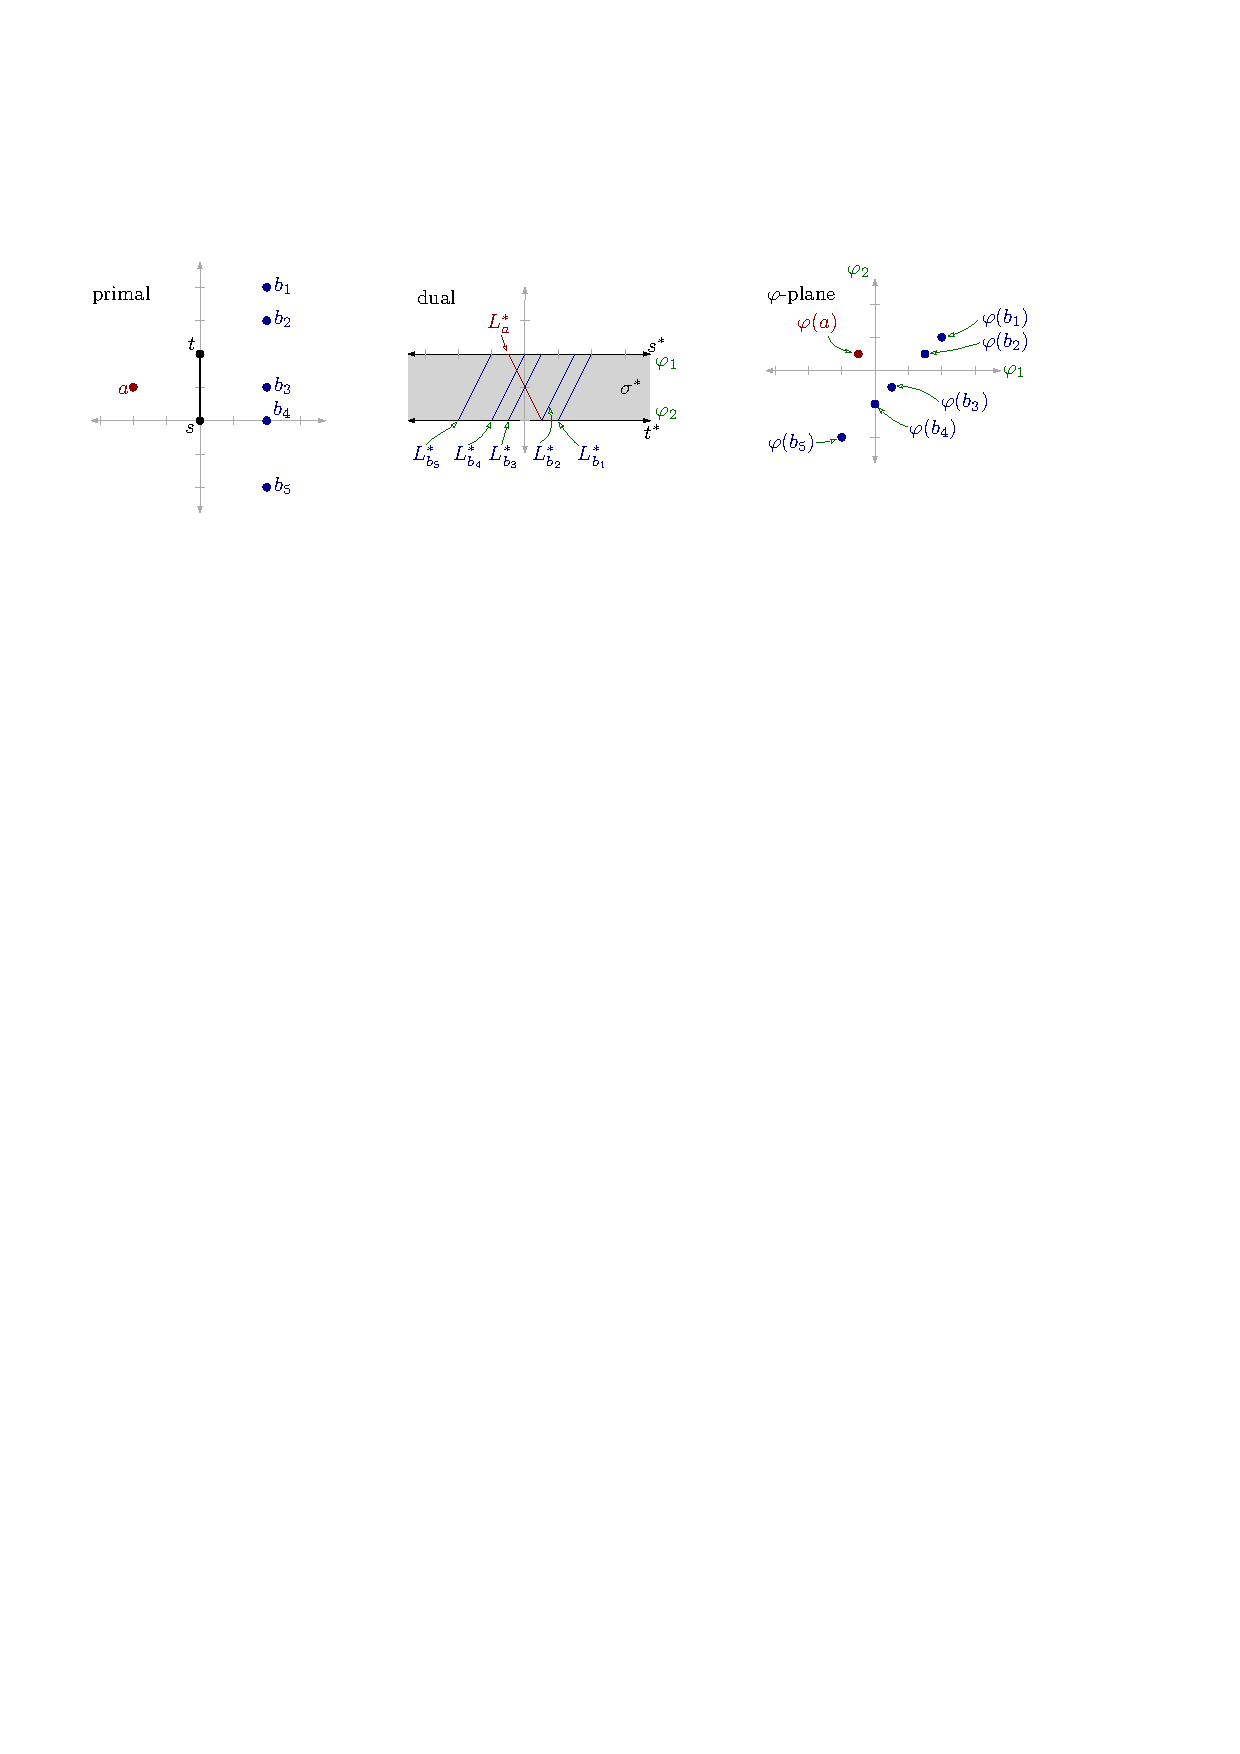
\includegraphics[scale=1.2]{pics/duality.pdf}}
\caption{.} 
\label{duality}
\end{figure}

\begin{proof}
Za potrebe dokaza uporabimo dualnost, opisano zgoraj.

Naj bo $\LL$ množica nevertikalnih premic, $\sigma^*$ pa množica točk dualnih nevertikalnim daljicam, ki sekajo daljico $\sigma$:

\[
		\sigma^* ~=~ \{ l^* \mid \ell\in \LL, \ell\cap \sigma\neq \emptyset\} 
\]

V dualnem prostoru je množica $\sigma^*$ $horizontal slab$

\[
		\sigma^* ~=~ \{ (m,-c)\in \RR^2\mid 0\le c\le s\}.
\]

\begin{figure}
\centerline{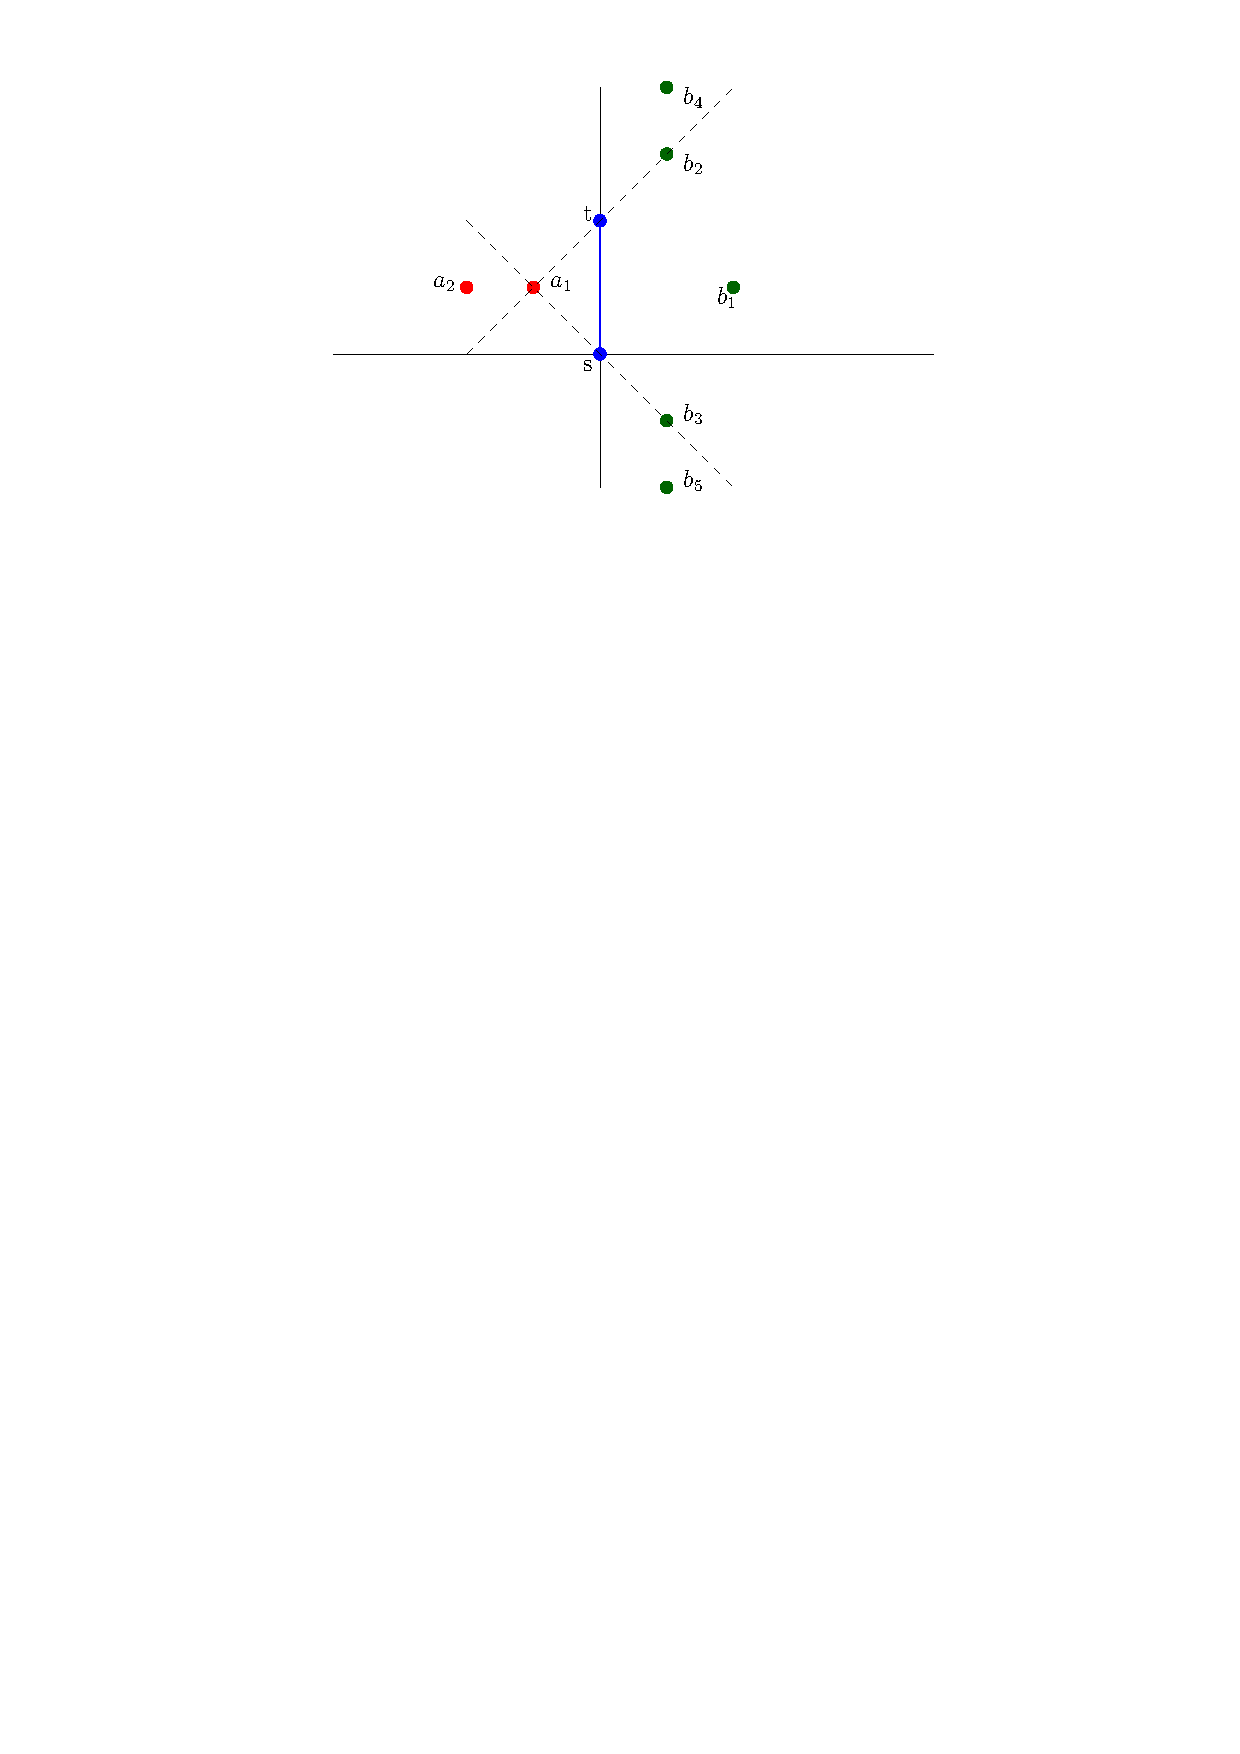
\includegraphics[scale=1.2]{pics/dual_problem3.pdf}}
\caption{Množici $A$ (rdeči točki) ter $B$ (zelene točke) levo in desno od daljice $st$ (zgornja slika). Črtkani črti predstavljata premici, čigar koeficienta sta uporabljena za izračun koordinat dualne točke $\varphi (a_1)$, predstavljata pa tudi vidno polje točke $a_1$.} 
\label{dualp}
\end{figure}

\begin{figure}
\centerline{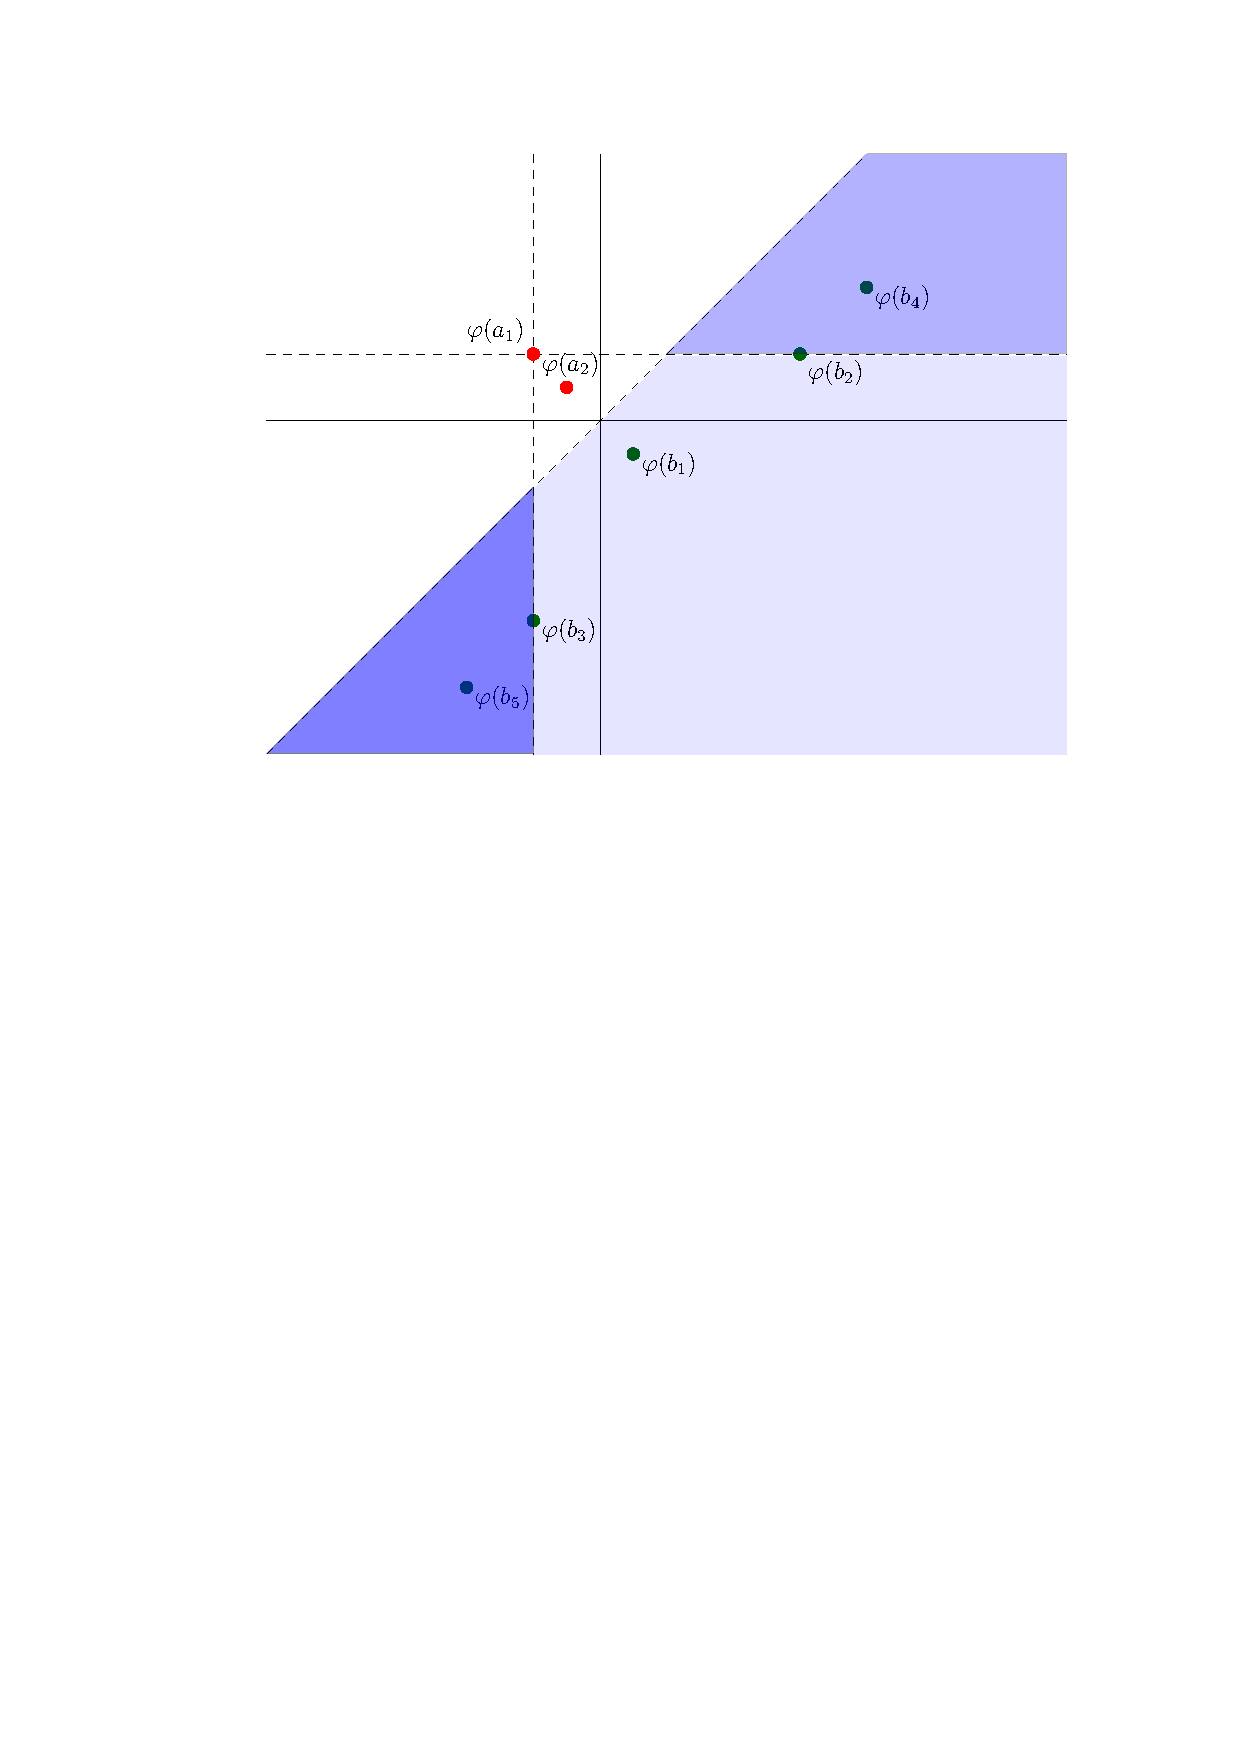
\includegraphics[scale=1.2]{pics/dual_problem4.pdf}}
\caption{Spodaj so prikazane točke iz slike ~\ref{dualp} v dualnem prostoru. Obarvano območje v sredini predstavlja prostor, v katerem se nahajajo vse take dualne točke $\varphi (b)$, za katere velja $b \in B(a_1)$. Obarvani območji levo in zgoraj predstavljata prostor dualnih točk $\varphi (b)$, za katere velja, da je presečišče premice $a_1b$ z osjo $y$ pod oziroma nad daljico $st$.} 
\label{dualp2}
\end{figure}


Za vsako točko $b\in B$ naj bo $L^* _b$ množica točk, dualnih premicam, ki gredo skozi $b$ in sekajo $\sigma$:

\[
		L^*_b=\{ \ell^* \mid \ell\in \LL, b \in \ell, \text{ and } \sigma\cap \ell\not= \emptyset\}.
	\]

V dualnem prostoru je $L^* _b$ daljica, ki je popolnoma vsebovana v slabu in ima krajišči $(\varphi_1(b),0)$ in $(\varphi_2(b),s)$ na obeh njegovih mejah. $\varphi_1(b)$ predstavlja smerni koeficient premice, ki seka točki $(0,s)$ in $b$, $\varphi_2(b)$ pa smerni koeficient premice, ki seka točki $(0,0)$ in $b$.

Definirajmo točko preslikave $\varphi(b)=(\varphi_1(b),\varphi_2(b))$. Funkcija preslikave $\varphi$ torej preslika točke na desni strani koordinatne osi $y$ v točke v ravnini.

Za vsak $b\in B$ velja neenakost $\varphi_1(b) \geq \varphi_2(b)$. Točke $B$ lahko razdelimo v tri skupine glede na predznaka koordinat točke preslikave $\varphi(b)$ in za vsako skupino je neenakost očitna:

\begin{align*}
    b_1 \in \{ (x,y) \mid (x,y) \in B, y < 0 \} \Rightarrow \varphi_1(b),\varphi_2(b) < 0 \text{ and } \varphi_1(b) > \varphi_2(b) \\
b_2 \in \{ (x,y) \mid (x,y) \in B, 0 <= y < s \} \Rightarrow \varphi_1(b) > 0, \text{ } \varphi_2(b) < 0 \\
    b_3 \in \{ (x,y) \mid (x,y) \in B, y >= s \} \Rightarrow \varphi_1(b) > 0, \text{ } \varphi_2(b) >= 0 \text{ and } \varphi_1(b) > \varphi_2(b)
\end{align*}

Enakost velja le v primeru, ko sta premici, ki definirata obe koordinati, isti. Do slednjega pride pri točkah $b$ s koordinato $x$ enako $0$. 

Iz zgornje neenakosti sledi, da točke preslikave $\varphi(b)$ vedno ležijo na polravnini $x \geq y$ in da je smerni koeficient premice, na kateri leži daljica $L^*_b$, nepozitiven. Podobno lahko ugotovimo, da za vsak $a \in A$ točka $\varphi(a)$ leži na polravnini $\varphi_2(a) > \varphi_1(a)$ in da ima premica, na kateri leži daljica $L^*_a$, pozitiven smerni koeficient.

Naj bo $a \in A$ in $b \in B$. Daljica $ab$ seka daljico $\sigma$ natanko takrat, ko $L^*_a$ seka $L^*_b$, ker daljico $ab$ v dualnem prostoru predstavlja ravno presečišče $L^*_a$ in $L^*_b$. Iz tega sledi naslednja lastnost:

\begin{align*}
		ab \cap \sigma \neq \emptyset ~\Longleftrightarrow ~ 
		(\varphi_1(a)-\varphi_1(b)) \cdot (\varphi_2(a)- \varphi_2(b)) < 0\\
				&	\varphi_1(a) <= \varphi_1(b)\\
				&	\varphi_2(a) >= \varphi_2(b).
\end{align*}
Z drugimi besedami: za točko $a \in A$ množico točk $b \in B$, kjer $ab$ seka $\sigma$, sestavljajo točke $b$, pri katerih se $\varphi(b)$ nahaja v drugem kvadrantu koordinatnega sistema z izhodiščem $\varphi(a)$. (Bolj natančno, gre za točke $\varphi(b)$, ki se nahajajo v preseku drugega kvadranta omenjenega koordinatnega sistema s polravnino $x \geq y$. Glej sliko.)

Za shranjevanje množice točk $\varphi(B)$, kjer je vsaka točka $b \in B$ asociirana s točko preslikave $\varphi(b)$, lahko uporabimo dvodimenzionalno območno drevo. Za vsako točko poizvedbe $a \in A$ lahko točke $b \in B$, kjer $ab$ seka $\sigma$, dobimo s poizvedbo na območnem drevesu, ki vrne točke $\varphi(B)$ v kvadrantu

\[
		\{(x,y)\mid  \varphi_1(a) < x \text{ and } \varphi_2(a) > y\}.
	\]
Območna drevesa so bolj podrobno opisana v poglavju x.

\end{proof}

\begin{lema}
\label{lema4}
$\Phi_\sigma(A,B)$ lahko izračunamo v času $\OO (n\log^4 n)$.
\end{lema}

\begin{proof}
Zgradimo množice $\{B_1,...,B_t\}$ in podatkovno strukturo $\D (B)$, opisano v lemi ~\ref{dualnost}. Za vsak $B_j$, kjer $j = 1,...,t$, zgradimo podatkovno strukturo, opisano v lemi ~\ref{lema1}. Ker velja $\sum_{i=1}^t |B_i|\log |B_i| = \OO (n\log n)$, potrebujemo za to
\[
		\sum_{i=1}^t O(|B_i| \log |B_i|) ~=~ O(n\log^2 n)
	\]

časa.

Obravnavajmo poljubno točko $a \in A$. Naredimo poizvedbo na $\D (B)$, ki nam vrne množico indeksov $I(a)$, za katero velja
\[
		B(a) ~=~ \bigcup_{i\in I(a)} B_i.
	\]

Za vsak $i\in I(a)$ naredimo poizvedbo s točko $a$ nad podatkovno strukturo, asociirano z $B_i$, da dobimo

\[	
		b_i^*(a) \in \arg\min \{ w_b \mid b\in B_i,~|ab|\le 1\}.
	\]

Potem velja
\begin{align*}
\min \{ w_b \mid b\in B_{\le 1}(a)\} ~=~ \min \{ w_{b_i^*(a)}\mid i\in I(a) \},
\end{align*}
s čimer lahko dobimo $\Phi_\sigma(a,B)$ iz točk $b_i^*(a)$, $i\in I(a)$.

Za točko $a$ potrebujemo $\OO (\log^2 n)$ časa, da izračunamo $I(a)$, in nato $\OO (\log^2 n)$ časa za vsak indeks $i$ v $I(a)$. Skupna časovna kompleksnost za vsako točko $a\in A$ je tako $\OO (\log^4 n)$.
\end{proof}

\subsection{Sekanje nepremične daljice}

Naj bo $G(P)$ neutežen graf nad množico točk $P$ (v nadaljevanju samo $G$), in naj bo $d_G(r,p)$ dolžina najkrajše poti v $G$ med $r$ in $p$.

Za vsako točko $r\in P$ naj bo $T_r$ drevo najkrajših poti v $G$ iz $r$. S $T_r[p]$ označimo pot v $T_r$ iz $r$ v $p$. $E_r$ naj bo množica povezav v $G$, ki se ne pojavijo v $T_r$. Velja torej $E_r = E(G)\setminus E(T_r)$.

Za vsak $r$ in $p$ v $P$ naj bo $\gamma(r,p)$ poligonalna pot, definirana s $T_r[p]$. Za vsak $r$ in vsako povezavo $pq\in E_r$ naj bo $\gamma (r,pq)$ zaprta poligonalna pot, ki jo dobimo z združitvijo $\gamma(r,p)$, $pq$ in  potjo, nasprotno $\gamma(r,q)$. Z $\length(r,pq)$ definiramo število povezav v $\gamma(r,pq)$. Tako velja $\length(r,pq) = d_G(r,p) + d_G(r,q) + 1$.

Naj bo $\sigma$ daljica, za katero predpostavimo, da ne vsebuje nobene točke iz $P$. Za vsako poligonalno pot $\gamma$ naj bo $X(\gamma, \sigma)$ število presečišč $\gamma$ s $\sigma$ po modulu 2. Za vsak $r,p\in P$ definiramo $N(r,p) = X(\gamma(r,p), \sigma)$ ter za vsak $r\in P$ in $pq\in E_r$ definiramo $N(r,pq) = X(\gamma(r,pq), \sigma)$.

Definirajmo sledeč optimizacijski problem:
\begin{align*}
	\Psi_\sigma(P) := \min ~~& \length(r,pq)\\
	 \mbox{s.t.}~~ & r\in P\\
				&	pq\in E_r\\
				&	N(r,pq)=1. 
\end{align*}

Iz rezultatov Cabella in Giannopoulosa (referenca!) sledi naslednje:

\begin{izrek}
Naj bo $(r^\star, p^\star g^\star)$ optimalna rešitev problema $\Psi_\sigma(P)$. Potem so točke v $T_{r^*}[p]\cup T_{r^*}[q]$ optimalna rešitev problema ločevanja s krogi. 
\end{izrek}

Za izračun $\Psi_\sigma(P)$ iteriramo po točkah $r$, tako da definiramo tudi
\begin{align*}
	\Psi_\sigma(r,P) := \min ~~& d_G(r,p)+d_G(r,q) \\
	 \mbox{s.t.}~~ & pq\in E_r\\
				&	N(r,pq)=1. 
\end{align*}

Optimizacijski problem lahko potem definiramo kot
\[
	\Psi_\sigma(P) ~=~ 1+ \min_{r\in P} \Psi_\sigma(r,P).
\]
Fiksirajmo nek $r\in P$ in se osredotočimo na rešitev problema $\Psi_\sigma(r,P)$.

Izračunamo drevo najkrajših poti $T_r$. Skupaj z vsako točko $p\in P$ shranimo $d_G(r,p)$. Nato izračunamo vrednosti $N(r,p), p\in P$ s preprostim sprehodom od spodaj navzgor po $T_r$. Začnemo z inicializacijo $N_r[r] := 0$. Za vsako točko $p\in P$, čigar starš v $T_r$ je $p'$, potem velja $N_r[p] = N_r[p'] + |\sigma\cap pp'| \pmod 2$. Če torej $pp'$ seka $\sigma$, velja $N_r[p]=N_r[p']+1 \pmod 2$, sicer velja
$N_r[p]=N_r[p']$.

Predpostavimo, da je $\sigma$ navpična daljica s krajišči $(0,0)$ in $(0,s)$. Iskanje optimalne povezave $pq$ razdelimo na tri primere:

\begin{itemize}
\item $pq$ ima obe krajišči na isti strani osi $y$, za kateri velja $N(r,p) \neq N(r,q)$, ali
\item $pq$ ima krajišči na različnih straneh osi $y$, $N(r,p) \neq N(r,q)$ in $pq$  ne seka $\sigma$, ali
\item $pq$ ima krajišči na različnih straneh osi $y$, $N(r,p) \neq N(r,q)$ in $pq$ seka $\sigma$.
\end{itemize}

\begin{lema}
\label{lema6}
$\Psi_\sigma(r,P)$ lahko izračunamo v času $\OO (n\log^4 n)$.
\end{lema}

\begin{proof}
Za $i\in \{0,1\}$ naj bo $L_i$ podmnožica točk iz $P$ levo od osy $y$ in z $N(r,p) = i \pmod 2$. Očitno velja
\[
		P~=~ L_0\cup L_1\cup R_0\cup R_1.
\]

Naj bosta $\sigma_+$ in $\sigma_-$ poltraka na osi $y$, ki ju dobimo, če odstranimo $\sigma$. Z uporabo $d_G(r,p)$ kot utež točke $p\in P$ potem dobimo

\begin{align*}
		 \Psi_\sigma(r,P) ~=~ \min \{ &\Phi( L_0,L_1), \Phi( R_0,R_1),
										\Phi_{\sigma_+}( L_0,R_1), \Phi_{\sigma_+}( L_1,R_0),\\
										&\Phi_{\sigma_-}( L_0,R_1), \Phi_{\sigma_-}( L_1,R_0),
										\Phi_{\sigma}( L_0,R_0), \Phi_{\sigma}(L_1,R_1) \}.
\end{align*}

Vsako posamezno instanco lahko izračunamo s pomočjo lem ~\ref{lema2} in ~\ref{lema4}v času $\OO (n\log^4 n)$.
\end{proof}

\begin{izrek}
Problem minimalnega ločevanja s krogi lahko rešimo v času $\OO (n^2\log^4 n)$.
\end{izrek}
\begin{proof}
Za vsak $r\in P$ izračunamo drevo najkrajših poti $T_r$ v $G$ iz $r$, razdalje $d_G(r,p), p\in P$ in paritete $N(r,p)$. Potem rešimo $\Psi_\sigma(r,P)$ s pomočjo leme ~\ref{lema6}.

TODO
\end{proof}

\chapter{Implementacija algoritma}
\label{ch3}


\section{SSSP drevo}

Algoritem za izgradnjo drevesa SSSP smo implementirali z mislijo na možnost njegove neposredne uporabe v algoritmu za ločevanje z diski. Posledično smo spustili nekaj funkcionalnosti dreves, ki jih kasneje v programu ne potrebujemo, po drugi strani pa dodali stvari, ki se ne tičejo drevesa, so pa potrebne kasneje. Tako na primer ne moremo dostopati do otrok vozlišč drevesa, po drugi strani pa pri dodajanju točk k drevesu te sproti tudi uvrstimo v eno izmed množic $L0$, $L1$, $R0$ in $R1$.

Za implementacijo smo uporabili razred $SSSPTree$ s štirimi zasebnimi atributi. Vsi so seznami točk tipa vector in vsaka hrani eno izmed omenjenih množic. Konstruktor kot vhodne parametre sprejme seznam točk $P$, točko izvora $r$ in daljico $st$ ter zgradi drevo. Metoda $getAllSets$ v seznamu vrne vse štiri atribute.

\subsection{Dodatki v razredu Point\texttt{\_}2}
Algoritem zgradi drevo implicitno. To pomeni, da kot rezultat ne dobimo nobene nove strukture, ampak konstruktor vsako točko doda v enega od štirih seznamov in pri tem spremeni vrednost dveh njenih atributov:

\begin{itemize}
\item dist: hrani razdaljo do korena drevesa in je tipa $unsigned\texttt{\_}int$
\item parent: hrani svojega starša in je tipa deljen kazalec ($ang.$ shared pointer) - zakaj že shared???
\end{itemize}

Noben imed omenjenih atributov ni del razreda $Point\texttt{\_}2$ v CGAL, zato smo jih sami dodali. S pomočjo kazalca na starša se je tako od vsake točke drevesa možno sprehoditi do korena, nasprotno pa to ne velja.

\subsection{Voronoijev diagram za iskanje najbližjega soseda}

Kot smo omenili pri opisu algoritma v prejšnjem poglavju, pri gradnji množice $W_i$ točke kandidatke testiramo tako, da poiščemo njihove najbližje sosede v množici $W_{i-1}$. Nad slednjo zgradimo VD, točke kandidatke pa uporabimo za poizvedbe nad tako strukturo.

Vse potrebne objekte in funkcije nam nudi že CGAL. Nad objektom razreda Voronoi\texttt{\_}Diagram\texttt{\_}2 lahko delamo poizvedbe s funkcijo locate(Point\texttt{\_}2 q), ki vrne objekt tipa Locate\texttt{\_}result. Za slednjega je potrebno ugotoviti, v katerega izmed treh tipov objekta, ki so del strukture VD, se ga da pretvoriti: lice, vozlišče ali enosmerno povezavo. Ker kot rezultat hočemo vrniti VD središče, ga moramo dobiti prek takega objekta. Razred tipa Face\texttt{\_}handle ima funkcijo $dual$, ki vrne vozlišče v DT, dualno takemu licu. Prek vozlišča VD lahko pridemo do dualnega lica v DT in nato iteratorja vozlišč, ki ga definirajo. Enosmerna povezava Halfedge\texttt{\_}handle ima funkciji $up$ in $down$, ki vrneta vozlišče v DT, dualno licu v VD nad oziroma pod povezavo.

Da dobimo dejanski objekt tipa Point\texttt{\_}2, ki definira vozlišče v DT oziroma središče v VD, uporabimo funkcijo $point()$. Na koncu moramo samo še preveriti evklidsko razdaljo med dobljeno točko in točko poizvedbe.

Opisano proceduro smo združili pod funkcijo $query$ in jo dodali v našemu razredu $VoronoiDiagram$, razširjenem nad Voronoi\texttt{\_}Diagram\texttt{\_}2. Koda funkcije $query$ je prikazana spodaj.

\lstinputlisting[language=C++, firstline=63, lastline=86]{VoronoiDiagram.h}

Kot vidimo v kodi, metoda poleg najbližjega soseda vrne tudi spremenljivko logičnega tipa, ki nam pove, če je razdalja med točko poizvedbe in njenim najbližjim sosedom manjša ali enaka 1. 

Naš razred ima še eno dodatno funkcijo. $Voronoi\texttt{\_}Diagram\texttt{\_}2$ omogoča vstavljanje samo objektov tipa $Site\texttt{\_}2$ (in $Point\texttt{\_}2$, ker zna CGAL samodejno pretvarjati med obema tipoma). Za potrebe drevesa SSSP smo v razredu $VoronoiDiagram$ omogočili tudi vstavljanje objektov tipa $Delaunay\texttt{\_}Vertex\texttt{\_}Handle$, iz katerega je moč enostavno dostopati do točke tipa $Point\texttt{\_}2$.
\subsection{Izgradnja drevesa} 

Konstruktor najprej zgradi DT nad $P$. Nato za izvorno točko $r\in P$ s pomočjo metode $locate$ poišče vozlišče v DT, s katerim sovpada. Pri tem preventivno preveri, da je tip rezultata, ki ga vrne $locate$, resnično \\ 
$Delaunay\texttt{\_}Vertex\texttt{\_}Handle$, sicer $r\notin P$. Za vse točke v $P$ velja predpostavka, da sta vrednosti njihovih atributov $dist$ in $parent$ ponastavljeni. Velja torej $\forall p\in P:$ $p.dist = \infty$ $\wedge$ $p.parent = nullptr$. 

Za generatorja točk kandidatk uporabljamo objekt tipa $deque$, primeren za hranjenje elementov v vrsti. Manjša razlika se potem pojavi pri dostopanju do točk v vrsti. V psevdokodi algoritma (vrstica 13) je $q$ poljubna točka v $Q$, medtem ko je v kodi $q$ vedno prva točka v vrsti (priklicana z metodo $front$, $pop\texttt{\_}front$ pa jo nato tudi odstrani iz vrste). Za $W_i$ in $W_{i-1}$ v zanki hranimo seznam Delaunayevih vozlišč (objekte tipa $Vertex\texttt{\_}Handle$). Voronoijev Diagram tipa $VoronoiDiagram$ zgradimo s seznamom $W_{i-1}$.

Povezave oziroma sosede točke $q$ najdemo s pomočjo metode v DT \\ $incident\texttt{\_}vertices(q)$. Ker ima v CGAL implementaciji DT poleg standardnih vozlišč še eno neskončno vozlišče, ki je sosedno vsem ostalim, takega soseda ne obravnavamo. Za ostale sosede $p$ najprej preverimo, če je njihova razdalja do $r$ $\infty$ (oziroma bolj konkretno, enaka numeric\texttt{\_}limits$\langle$int$\rangle$ ::max()), potem pa poiščemo njihovega najbližjega soseda $w$ v $W_{i-1}$ z metodo $query$ našega razreda $VoronoiDiagram$. Če $|pw| <= 1$, naredimo naslednje:

\begin{itemize}
\item $p.setDist(i)$
\item $Q.insert(p)$
\item $Wi.insert(p)$
\item $p.setParent(shared\texttt{\_}ptr\langle Point\texttt{\_}2\rangle  $ $w)$
\item $p.setNr(updateNr(w,$ $p,$ $st))$
\item $categorize(p,$ $st)$
\end{itemize}

Zadnji dve točki nista omenjeni v psevdokodi, ker njuna uporabnost pride v poštev šele kasneje pri separaciji z diski. $updateNr$ vrne novo vrednost za atribut $nr$ točke $p$. Funkcija preveri, če daljica $pw$ seka $st$ in če jo, vrne $(w.getNr() + 1)$ $\%$ $2$, sicer vrne $w.getNr()$. $categorize$ točko $p$ na podlagi njenega atributa $nr$ in relativnega položaja glede na $st$ (ki je ali levo ali desno) doda v enega od štirih seznamov l0, l1, r0 ali r1.

\section{Drevo najbližjega soseda}

\begin{figure}
\centerline{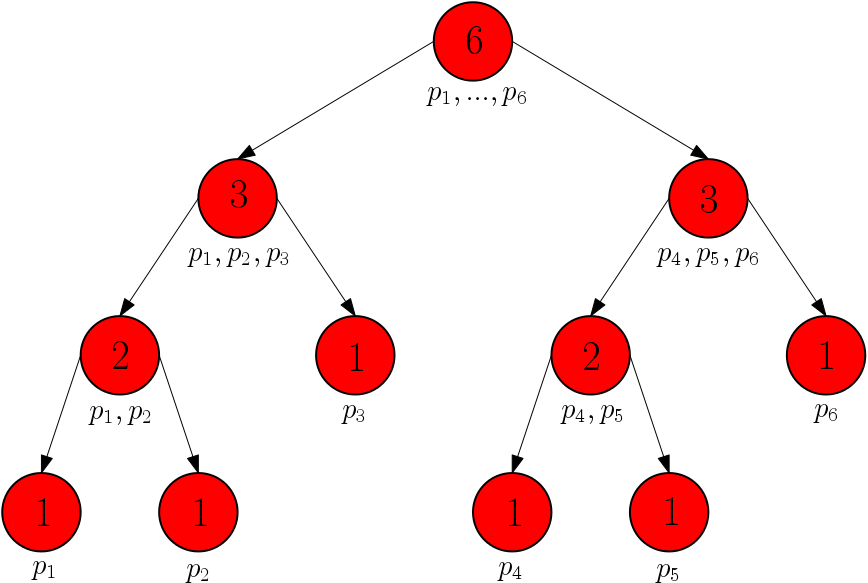
\includegraphics[scale=0.5]{pics/nntree-png.png}}
\caption{Drevo najbližjega soseda, ki hrani 6 točk, prikazano v drevesni strukturi. Vrednosti vozlišč ponazarjajo število točk, shranjenih v objektu, ki omogoča poizvedbe najbližjega soseda, pod vozlišči pa so nanizane konkretne točke.}
\label{nntree}
\end{figure}

\begin{figure}
\centerline{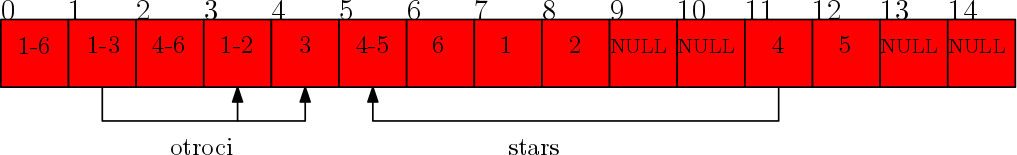
\includegraphics[scale=0.5]{pics/nnarray-png.png}}
\caption{Drevo najbližjega soseda, ki hrani 6 točk, predstavljeno v obliki seznama. Za vsako celico so prikazani indeksi točk, ki jih hrani objekt v njej.}
\label{nnarray}
\end{figure}

Drevo najbližjega soseda, opisano v poglavju 3.3, bi lahko implementirali s kazalci ali seznamom. Odločili smo se slednjega. Seznam hrani kazalce ($shared{\_}ptr$) na objekte podatkovne strukture $DS(P(\nu))$ za poizvedbe najbližjega soseda. Velikost seznama, ki hrani $n$ točk, je enaka $2^{\lceil \log_2n \rceil+1}-1$. Nekatera vozlišča na najnižjem nivoju drevesa so lahko tudi prazna (torej brez objektov). Primer takega drevesa je prikazan na sliki ~\ref{nntree}. Otroka vozlišča, ki se v seznamu nahaja na mestu $i$, se nahajata na mestu $2i+1$ in $2i+2$. Podobno se starš vozlišča na mestu $i$ nahaja na mestu $\lfloor(i-1)/2\rfloor$.



Za podatkovno strukturo s poizvedbami najbližjega soseda smo sprva hoteli uporabiti VD, vendar smo se kasneje odločili za Kd drevo. Razlog za to je implementacija VD v knjižnici CGAL. Ker je prostorska kompleksnost VD $\OO(n)$, bi pričakovali, da poraba prostora raste linearno z večanjem VD. Izkaže se, da je rast počasnejša od linearne, kar pomeni, da na primer 100 VD objektov velikosti 10 porabi več prostora kot 10 objektov velikosti 100. Posledično poraba prostora ni enaka za vsak nivo drevesa, temveč z globino raste. Razlike se v celotnem algoritmu potem še potencirajo, ker zgradimo VD v (skoraj) vsakem vozlišču drevesa najbližjega soseda, vsako tako drevo pa v vsakem vozlišču sekundarnega drevesa v območnem drevesu. Ko smo testirali implementacijo Kd dreves v CGAL, smo ugotovili tudi, da je čas konstrukcije bistveno krajši kot pri VD. Primerjave med konstrukcijama obeh podatkovnih struktur (procesorski čas in poraba RAM-a) so prikazane v poglavju Rezultati.

\subsection{Kd drevo}

Kot osnovo smo za poizvedbe najbližjega soseda uporabili funkcijo $search$ v razredu $Kd{\_}tree$, ki kot argument sprejme $OutputIterator$, kamor se shranjujejo objekti, ki jih poizvedba vrne, in $FuzzyQueryItem$, ki je v dvodimenzionalnem primeru lahko krog ali pravokotnik in določa območje iskanja. Kot argument lahko sprejme vrednost $\epsilon$, ki določa stopnjo mehkosti (ang. fuzzyness) in se jo uporablja pri aproksimacijskih poizvedbah, ki pa jih v našem algoritmu nismo potrebovali. Časovna kompleksnost funkcije $search$ je enaka $\OO(\log n + k)$, kjer je $k$ število vrnjenih točk znotraj območja iskanja. Ker naš algoritem zahteva $\OO(\log n)$, smo razredu $Kd{\_}tree$ dodali podobno funkcijo, ki pa iskanje zaključi v istem trenutku, ko ugotovi, da se vsaj ena točka nahaja znotraj območja iskanja. Če na primer za neko notranje vozlišče Kd drevesa ugotovi, da vse točke v njegovem poddrevesu ustrezajo kriterijem iskanja, jih ne doda enega po enega v $OutputIterator$, temveč doda samo "dummy" točko in zaključi. Če najde samo eno točko (ko pride do lista Kd drevesa), potem tako točko tudi vrne. To si lahko privoščimo, ker nas v notranjih vozliščih drevesa najbližjega soseda ne zanimajo konkretne točke, ampak samo informacija, ali se vsaj ena točka nahaja v območju iskanja. Šele ko pridemo do lista NN drevesa, nas zanima konkretna točka. S tem, ko je vedno vrnjena ena točka, se časovna kompleksnost spremeni v $\OO(\log n)$.

\section{Implementacija optimizacijskega problema $\Phi_\sigma(A,B)$}

Za rešitev optimizacijskega problema, predstavljenega v poglavju ~\ref{opt2}, smo uporabili implementacijo območnih dreves v CGAL, za uporabo dualnosti pa napisali lasten razred (bolj natančno $struct$) $DualPoint$ za točke v dualnem prostoru.

\subsection{DualPoint - implementacija dualne točke}

Odločili smo se razlikovati po tipu med navadnimi točkami in točkami v dualnem prostoru, ki izhajajo iz premic v primarnem prostoru. Razred $DualPoint$ hrani dva atributa. Prvi je točka v dualnem prostoru tipa $Point\texttt{\_}2$, poimenovan $point$. Drugi je kazalec na točko tipa $Point\texttt{\_}2$, poimenovan $originalPoint$. Če $point$ predstavlja točko $(\varphi_1(b), \varphi_2(b))$ (glej poglavje ~\ref{opt2}), potem $originalPoint$ predstavlja točko $b$. Konstruktor razreda kot argumenta sprejme točko $b$ in daljico $\sigma$ in s pomočjo funkcije $imagePoint$ izračuna točko preslikave.


\subsection{Območno drevo}
Za dvodimenzionalna območna drevesa smo uporabili implementacijo v knjižnici CGAL, ki jo predstavlja razred $Range\texttt{\_}tree\texttt{\_}2$. Vsako vozlišče hrani par $<kljuc, vrednost>$. Vrednost dodatno opisuje vozlišče in je lahko tudi prazna, ključ pa se uporablja pri izgradnji drevesa in poizvedbah. Oba argumenta sta v razredu podana kot $template$, kar pomeni, da moramo pri konstrukciji drevesa zanju podati konkretna tipa. 
Za ključ smo uporabili naš razred $Dual\texttt{\_}Point$, kot vrednost pa vsako vozlišče hrani svoje drevo NN.

Pri inicializaciji drevesu podamo seznam parov dualnih točk in praznega drevesa NN. Nato se iterativno sprehodimo po prvem nivoju drevesa (primarnem drevesu) - tako kot pri preiskovanju v širino - s funkcijo $traverse\texttt{\_}and\texttt{\_}populate\texttt{\_}with\texttt{\_}data$. Za vsako vozlišče pokličemo funkcijo $build\texttt{\_}NN\texttt{\_}Tree\texttt{\_}on\texttt{\_}layer2$, ki rekurzivno  od spodaj navzgor za vsako vozlišče v sekundarnem drevesu, na katerega kaže vozlišče v primarnem drevesu, vstavi v (v tistem trenutku prazno) njegovo drevo NN točke, ki jih hranita drevesi NN njegovih otrok. Pri listih je v drevo NN vstavljena točka, čigar dualna točka je uporabljena kot ključ vozlišča. Rekurzivni klic funkcije se torej kliče pred vstavljanjem točk v drevo NN. S pomočjo rekurzije je vsakemu notranjemu vozlišču v sekundarnem drevesu seznam točk v njegovem poddrevesu, ki ga potrebujemo za izgradnjo njegovega drevesa NN, implicitno podan preko dreves NN njegovih otrok. Če bi drevesa NN gradili od zgoraj navzdol v sekundarnem drevesu, bi morali za vsako vozlišče narediti sprehod po njegovem poddrevesu. V primarnem drevesu so vsa drevesa NN prazna.

\subsubsection{Poizvedbe v območnem drevesu}
Razredu $Range\texttt{\_}tree\texttt{\_}d$ smo za poizvedbe dodali funkcijo $window\texttt{\_}query\texttt{\_}impl\texttt{\_}modified$, ki  kot osnovo uporablja obstoječo funkcijo $window\texttt{\_}query\texttt{\_}impl$. Argumenti funkcije so $OutputIterator$, kamor se vstavljajo vrnjene točke, interval $I$, ki ga definirata dve dualni točki, tretji argument, ki ga v obstoječi funkciji ni, pa je točka $a$, ki jo uporabimo za poizvedbe najbližjega soseda v drevesih NN. Pri dvodimenzionalnih območnih drevesih je geometrijska predstavitev intervala pravokotnik; levo krajišče intervala ustreza spodnjemu levemu oglišču pravokotnika, desno krajišče pa zgornjemu desnemu oglišču. Interval je zaprt. 

Če za vozlišče $w$ v primarnem drevesu ugotovimo, da njegovo celotno poddrevo ustreza pogojem poizvedbe, nadaljujemo s preiskovanjem v njegovem sekundarnem drevesu. Če za vozlišče $v$ v sekundarnem vozlišču ugotovimo, da so vsa vozlišča v njegovem poddrevesu vsebovana v intervalu $I$, ne dodamo vso poddrevo v rezultat, kot je to storjeno v osnovni funkciji, temveč opravimo še poizvedbo najbližjega soseda točke $a$ v drevesu NN vozlišča $v$. Za vsako obiskano vozlišče $w$ v primarnem drevesu prav tako preverimo, če je vsebovano v intervalu $I$. Če je temu tako, točko, iz katere izhaja dualna točka, ki predstavlja ključ vozlišča $w$, dodamo v seznam vrnjenih točk. Enako velja za obiskana vozlišča v sekundarnem drevesu. [To pomeni vsi listi v sekundarnem drevesu. Naj listi sploh hranijo kd drevo velikosti 1?] 


\lstinputlisting[language=C++, firstline=1, lastline=37]{KdTreeQuery.h}

\lstinputlisting[language=C++, firstline=1, lastline=33]{NNquery.h}

\section{Minimalno ločevanje}

\begin{figure}
\centerline{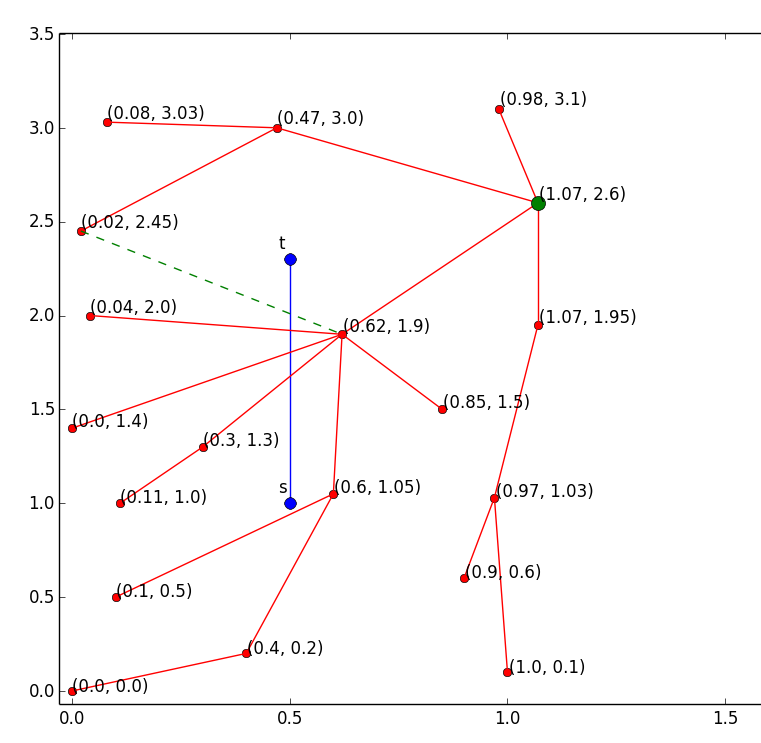
\includegraphics[scale=0.7]{pics/primer1.png}}
\caption{Dodaj primer množic L0, L1, R0, R1. }
\label{primer-sep}
\end{figure}


Za rešitev optimizacijskega problema $\Psi_\sigma(r,P)$ (glej lemo ~\ref{lema6}) smo napisali dve funkciji, ki rešita optimizacijska problema $\Phi(A,B)$ in $\Phi_\sigma(A,B)$.

\subsection{opt1}
Funkcija $findMinPair(S_i, S_{i+1}, currentMinWeight)$ reši optimizacijska problema $\Phi(L_0, L_1)$ in $\Phi(R_0, R_1)$. Parameter $currentMinWeight$ hrani trojko $(a, b, w_a + w_b)$, kjer točki $a$ in $b$ s povezavo $ab$ tvorita trenutno najbolj optimalno pot.

Nad točkami $p\in S_{i+1}$ zgradimo drevo $NN(S_{i+1})$. Za vsako točko $q\in S_i$ naredimo poizvedbo najbližjega soseda v drevesu, če je razdalja $q$ do korena drevesa $SSSP$ manjša od dolžine trenutno najbolj optimalne poti. Za točko $b$, ki jo vrne poizvedba, preverimo, če je vsota uteži $w_q + w_b$ manjša od $w_a+w_b$. Če je temu tako, posodobimo $currentMinWeight$ z $(q, b, w_q + w_b)$.

\subsection{opt2}
Funkcija $findminpairRi (L_i, L_j, R_i, currentMinWeight, st)$. Šest instanc problema $\Phi_\sigma(A,B)$ v $\Psi_\sigma(r,P)$ ne rešujemo neodvisno, ker bi sicer morali šestkrat konstruirati območno drevo. Probleme z isto podmnožico $R_i$ združimo pod skupni problem, ki ga s funkcijo rešimo na sledeč način.

Zgradimo območno drevo s točkami $p\in R_i$. Za vsako točko $p_i\in L_i$ naredimo poizvedbo v območnem drevesu, pri čemer za območje iskanja podamo  drugi kvadrant koordinatnega sistema, ki ima za izhodišče točko $\varphi (p_i)$. Levo krajišče tako predstavlja točka $(\varphi_1 (p_i), -\infty)$, desno pa točka $(\infty, \varphi_2 (p_i))$. Parameter $st$ predstavlja daljico $\sigma$, s katero lahko izračunamo dualne točke. Parameter $currentMinWeight$ hrani trojko $(a, b, w_a + w_b)$, kjer točki $a$ in $b$ s povezavo $ab$ tvorita trenutno najbolj optimalno pot, izračunano z do zdaj rešenimi optimizacijskimi problemi $\Phi$ in $\Phi_\sigma$. Za vse točke $q_k$, ki jih vrne poizvedba, preverimo, če je vsota uteži $w_{p_i} + w_{q_k}$ manjša od $w_a+w_b$. Če je temu tako, posodobimo $currentMinWeight$ z $(p_i, q_k, w_{p_i} + w_{q_k})$. 

Funkcijo smo optimizirali tako, da smo zmanjšali število poizvedb. Poizvedb ne delamo s točkami, pri katerih je razdalja do korena drevesa SSSP večja od vsote razdalj točk $a$ in $b$, ki tvorita trenutno optimalno zaprto pot. S poizvedbami nad drugim kvadrantom rešimo problem $\Phi_\sigma(L_i,R_i)$.

Funkcija potem nadaljuje s poizvedbami za vsako točko $p_j\in L_j$. Za vsak $p_j$ opravimo dve poizvedbi. Pri eni za območje iskanja podamo prvi kvadrant, pri drugi pa tretji kvadrant koordinatnega sistema, ki ima za izhodišče točko $\varphi (p_j)$. Za vse točke $q_l$, ki jih vrneta poizvedbi, nato zopet preverimo vsoto uteži $w_{p_j} + w_{q_l}$ in po potrebi posodobimo $currentMinWeight$.

S poizvedbami nad prvim kvadrantom rešimo problem $\Phi_{\sigma_+}(L_j,R_i)$, s poizvedbami nad tretjim kvadrantom pa problem $\Phi_{\sigma_-}(L_j,R_i)$. Glej tudi sliko ~\ref{dualp}. Območje iskanja v teoretičnem pogledu ne določajo samo kvadranti, temveč tudi polravnina $x \geq y$. Ampak presek obeh območij ni pravotnik, za območje iskanja v območnem drevesu pa ne moremo vzeti poljubnega poligona. Omejitev območja iskanja tudi ne prinaša nobenih prednosti. Vse točke $b\in B$ se nahajajo v omenjeni polravnini, točke na drugi strani polravnine, ki se nahajajo v prvem, drugem ali tretjem kvadrantu, pa pripadajo množici točk na levi strani osi $y$, ki niso shranjene v območnem drevesu.

Funkcija se izvede dvakrat, kar pomeni, da tudi območno drevo zgradimo dvakrat; enkrat za $R_0$ in enkrat za $R_1$. Za točke v $L_0$ in $L_1$ naredimo tri poizvedbe; po enkrat v prvem, drugem in tretjem kvadrantu.

\subsection{Kreiranje cikla}
Ko dobimo par točk $a, b\in P$, ki določata minimalno zaprto pot, ki ločuje točki $s$ in $t$, v seznam shranimo vse točke, ki tvorijo cikel. S pomočjo funkcije $getParent()$ lahko za vsako točko $p$ v drevesu $SSSP(r, P)$ dobimo njegovega starša in s tem pot $T_r[p]$ v obratnem vrstnem redu (z začetkom pri točki $p$ in koncem pri točki $r$), ki jo označimo kot $T_r^{-1}[p]$. Pot $T_r[p]$ brez točke $r$ označimo z $T_{r-1}[p]$. Cikel lahko potem dobimo z združitvijo dveh poti $T_r^{-1}[a] + T_{r-1}[b]$, s čimer dobimo pot $(a,...,r,...b)$. Vrnjen seznam predstavlja cikel, v katerem je začetna točka shranjena samo enkrat. Za dolžino najbolj optimalne poti se do konca izvajanja programa hrani vsota dolžin točk $a$ in $b$. Dolžina, ki jo program vrne kot rezultat, je povečana za 1.

\section{Obravnava posebnih vhodnih primerov}
Pri algoritmu ločevanja z diski smo večkrat omenili, da je za daljico $\sigma$ privzeto, da je vertikalna. Če želimo uporabiti algoritem na primeru, kjer daljica ni vertikalna, je potrebno vse vhodne točke predhodno rotirati 

točke, ki ležijo na y osi, grejo k b (preveri tip neskončne vrednosti v dualpoint)



\chapter{Rezultati}
\label{ch3}

\begin{figure}
\centerline{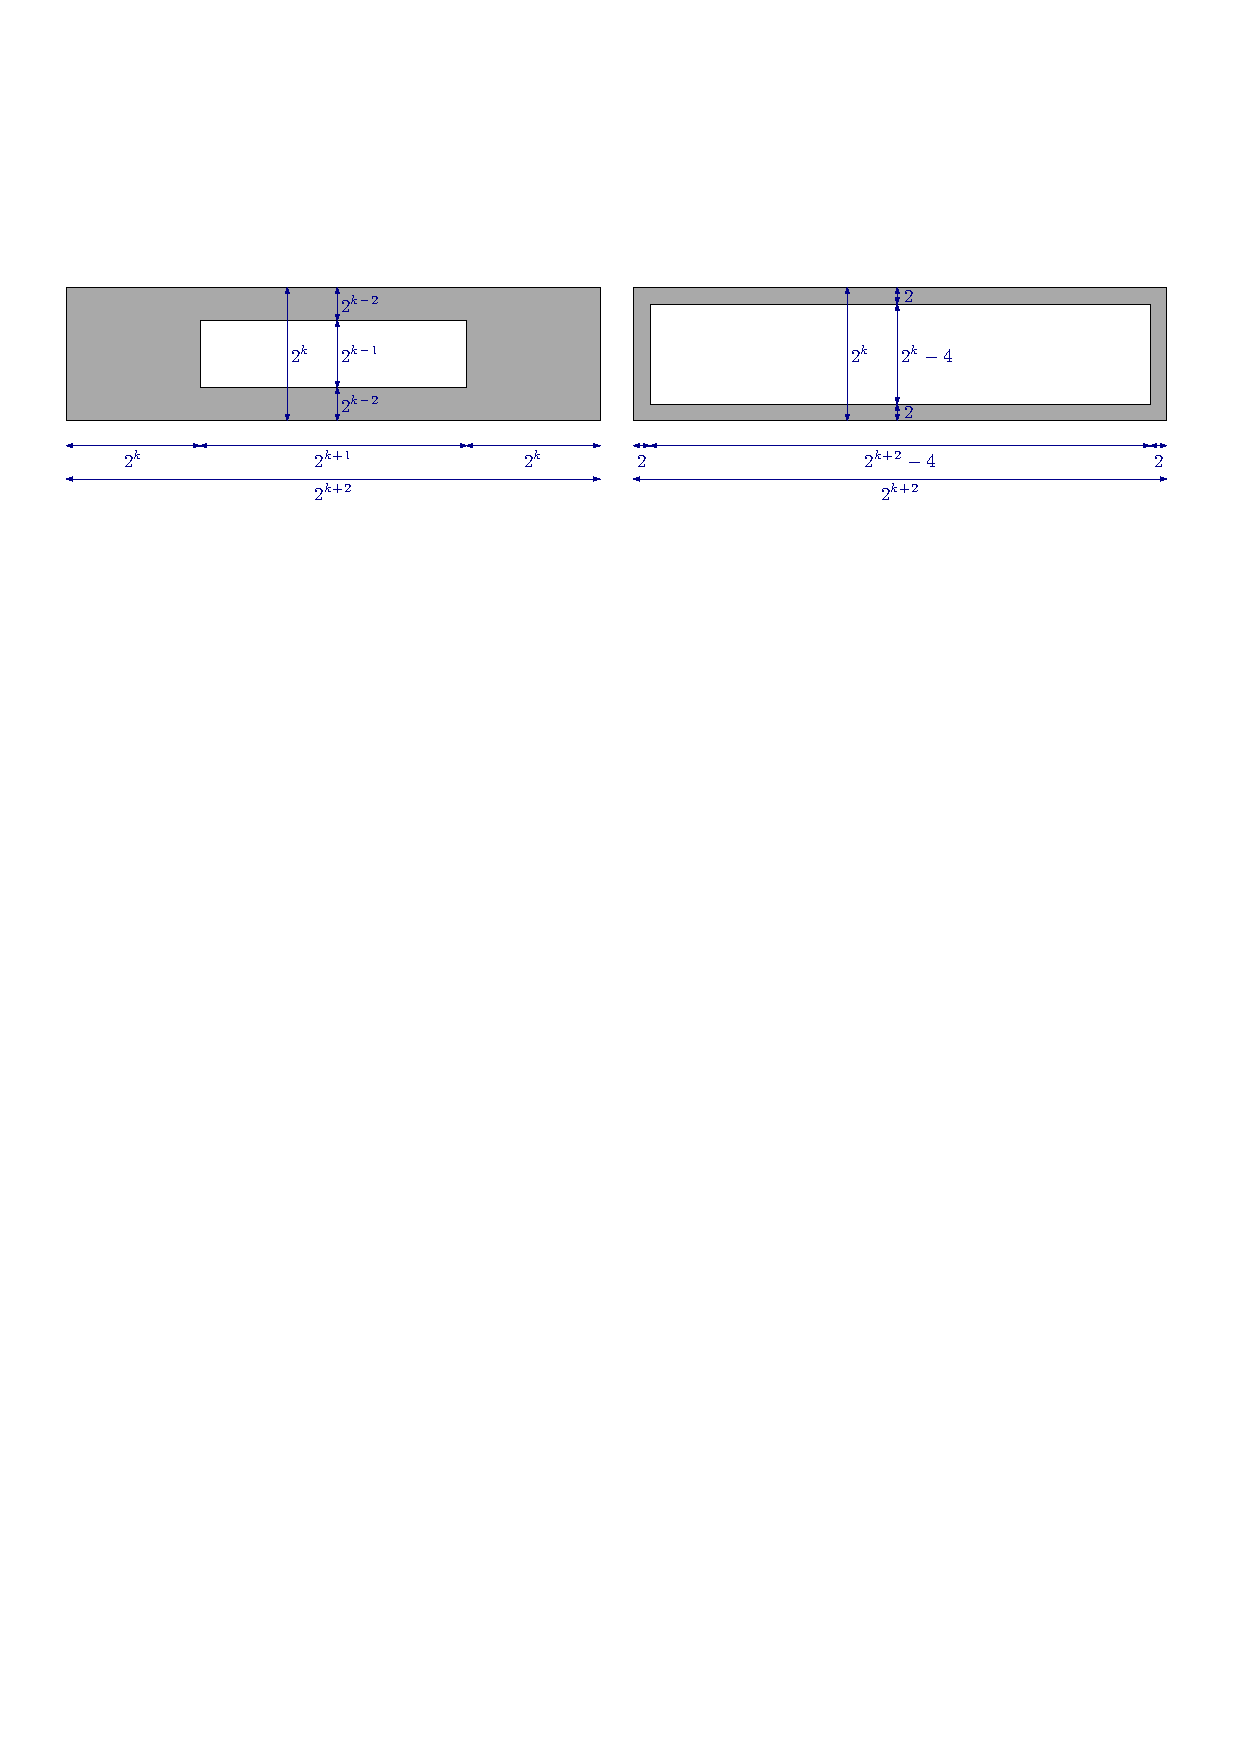
\includegraphics[scale=0.75, page=1]{pics/data_generation.pdf}}
\caption{. }
\label{generation}
\end{figure}

\begin{figure}
\centerline{\includegraphics[scale=0.75, page=2]{pics/data_generation.pdf}}
\caption{. }
\label{generation}
\end{figure}

\begin{table}
\begin{center}
\begin{tabular}{l|l|l|l|l|l|l}
\hline
number of točk & 50k & 100k & 250k & 500k & 750k & 1mio \\ \hline \hline
CPU(VD) [s] & 0.0859 & 0.196 & 0.562 & 1.2667 & 2.0495 & 2.9304 \\ \hline
CPU(kd drevo) [s] & 0.0025 & 0.0047 & 0.0126 & 0.025 & 0.0375 & 0.0497
\end{tabular}
\end{center}
\label{cpu_compare}
\caption{Časi konstrukcij Voronoijevega diagrama in kd drevesa v sekundah. Vsaka konstrukcija se je izvedla desetkrat, na podlagi tega pa se je izračunal povprečni čas izvedbe.}
\end{table}

\begin{table}
\begin{center}
\begin{tabular}{l|l|l|l|l|l|l}
number of točk & 50k & 100k & 250k & 500k & 750k & 1mio \\ \hline \hline
RAM(VD) [mb] & 7.2 & 14.4 & 34.3 & 68.9 & 103.6 & 137.9 \\ \hline
RAM(kd drevo) [mb] & 1.9 & 3.8 & 9.5 & 19 & 28.5 & 38.1
\end{tabular}
\end{center}
\label{ram_compare}
\caption{Velikost prostora v megabajtih, ki ga zasede en objekt Voronoijevega diagrama ali kd drevesa.}
\end{table}





\section{Drevo najkrajših poti}

\begin{table}
\begin{center}
\begin{tabular}{l*{3}{r}}
Pravokotnik brez lukenj & \multicolumn{3}{c}{20K točk}\\						
dimenzije pravokotnika	&	$4\times 1$	&	$8\times 2$	&	$16\times 4$ \\
\hline
predprocesiranje SSSP	&	0.025	&	0.027	&	0.025		\\
povprečje za koren s SSSP	&	0.131	&	0.130	&	0.127		\\
predprocesiranje BFS 	&	25.057	&	20.433	&	17.773		\\
povprečje za koren z BFS	&	3.406	&	1.359	&	0.404		\\
mreža	&	1.605	&	1.647	&	0.695	\vspace{.2cm}	\\

&	$32\times 8$	&	$64\times 16$	&	$128\times 32$	\\
\hline
predprocesiranje SSSP &	0.025	&	0.025	&	0.026 \\
povprečje za koren s SSSP &	0.126	&	0.129	&	0.136 \\
predprocesiranje BFS &	17.734	&	17.347	&	17.179 \\
povprečje za koren z BFS &	0.088	&	0.025	&	0.009 \\
mreža &	0.227	&	0.089	&	0.053 \vspace{.2cm} \\
\hline
  & \multicolumn{3}{c}{50K točk}  \\						
&	$4\times 1$	&	$8\times 2$	&	$16\times 4$ \\
\hline
predprocesiranje SSSP	&	0.091	&	0.091	&	0.070		\\
povprečje za koren s SSSP	&	0.592	&	0.562	&	0.375		\\
predprocesiranje BFS	&	$>$3min	&	159.812	&	144.965		\\
povprečje za koren z BFS	& omejitev RAM-a & 9.378	&	2.789		\\
mreža				&	11.567	&	13.660	&	4.592	\\

&	$32\times 8$	&	$64\times 16$	&	$128\times 32$	\\
\hline
predprocesiranje SSSP &	0.071	&	0.070	&	0.069 \\
povprečje za koren s SSSP &	0.377	&	0.372	&	0.366 \\
predprocesiranje BFS &	140.404	&	131.854	&	132.475 \\
povprečje za koren z BFS &	0.584	&	0.144	&	0.044 \\
mreža &	1.346	&	0.432	&	0.187
\end{tabular}
\caption{Times for shortest paths in Pravokotniks without luknje.}
\label{table1}
\end{center}
\end{table}



\begin{table}
\begin{center}
\begin{tabular}{l*{3}{r}}
Pravokotnik 1 small hole & \multicolumn{3}{c}{10K točk}\\						
dimenzije pravokotnika	&	$4\times 1$	&	$8\times 2$	&	$16\times 4$		\\
\hline
predprocesiranje SSSP	&	0.021	&	0.012	&	0.012		\\
povprečje za koren s SSSP	&	0.104	&	0.059	&	0.060		\\
predprocesiranje BFS	&	8.500	&	4.300	&	4.100		\\
povprečje za koren z BFS	&	1.183	&	0.318	&	0.091		\\
mreža	&	0.486	&	0.513	&	0.168  \vspace{.2cm}	\\
&	$32\times 8$	&	$64\times 16$	&	$128\times 32$ \\
predprocesiranje SSSP &	0.012	&	0.012	&	0.012 \\
povprečje za koren s SSSP &	0.061	&	0.064	&	0.070 \\
predprocesiranje BFS &	4.100	&	4.000	&	4.000 \\
povprečje za koren z BFS &	0.026	&	0.008	&	0.003 \\
mreža &	0.072	&	0.035	&	0.026\vspace{.2cm} \\
\hline
  & \multicolumn{3}{c}{20K točk}\\
  &	$4\times 1$	&	$8\times 2$	&	$16\times 4$		\\  			
\hline
predprocesiranje SSSP	&	0.027	&	0.026	&	0.025	\\
povprečje za koren s SSSP	&	0.142	&	0.137	&	0.136	\\
predprocesiranje BFS	&	24.813	&	19.817	&	18.396	\\
povprečje za koren z BFS	&	3.253	&	1.328	&	0.467	\\
mreža				&	2.181	&	2.627	&	0.668	\\
&	$32\times 8$	&	$64\times 16$	&	$128\times 32$ \\
predprocesiranje SSSP &	0.025	&	0.025	&	0.025	\\
povprečje za koren s SSSP &	0.136	&	0.138	&	0.145	\\
predprocesiranje BFS &	17.976	&	17.542	&	17.313	\\
povprečje za koren z BFS &	0.108	&	0.031	&	0.011	\\
mreža &	0.262	&	0.104	&	0.060 
\end{tabular}
\caption{Times for shortest paths in Pravokotniks with a small hole.}
\label{table2}
\end{center}
\end{table}

\begin{table}
\begin{center}
\begin{tabular}{l*{3}{r}}
Pravokotnik 4 small luknje & \multicolumn{3}{c}{10K točk} \\
dimenzije pravokotnika	&	$32\times 8$	&	$64\times 16$	&	$128\times 32$	\\						
\hline
SSSP preprocessing	&	0.021	&	0.018	&	0.018	\\
povprečje za koren s SSSP	&	0.056	&	0.058	&	0.064	\\
predprocesiranje BFS	&	6.291	&	6.102	&	6.364	\\
povprečje za koren z BFS	&	0.033	&	0.010	&	0.004	\\
mreža				&	0.064	&	0.031	&	0.023	\\
\hline
& \multicolumn{3}{c}{20K točk} \\
\hline
predprocesiranje SSSP &  0.027	&	0.026	&	0.026 \\
povprečje za koren s SSSP &	0.125	&	0.126	&	0.131 \\
predprocesiranje BFS &	18.325	&	17.887	&	17.256	\\
povprečje za koren z BFS & 0.102	&	0.031	&	0.010 \\
mreža &	0.230	&	0.096	&	0.055 
\end{tabular}
\caption{Časi za najkrajše poti v pravokotnikih s 4 manjšimi luknjami.}
\label{table4}
\end{center}
\end{table}


\begin{table}
\begin{center}
\begin{tabular}{l*{3}{r}}
Pravokotnik 4 večje luknje & \multicolumn{3}{c}{5K točk} \\
dimenzije pravokotnika	&	$32\times 8$	&	$64\times 16$	&	$128\times 32$ \\						
\hline
predprocesiranje SSSP	&	0.007	&	0.009	&	0.009	\\
povprečje za koren s SSSP	&	0.027	&	0.028	&	0.026	\\
predprocesiranje BFS	&	1.420	&	1.420	&	1.390	\\
povprečje za koren z BFS	&	0.007	&	0.003	&	0.002	\\
mreža				&	0.019	&	0.013	&	0.010	\\
\hline
& \multicolumn{3}{c}{10K točk} \\
\hline
predprocesiranje SSSP &	0.012	&	0.018	&	0.019	\\
povprečje za koren s SSSP &	0.057	&	0.054	&	0.053	\\
predprocesiranje BFS &	5.740	&	5.660	&	5.720	\\
povprečje za koren z BFS &	0.028	&	0.013	&	0.007	\\
mreža &	0.060	&	0.038	&	0.027 
\end{tabular}
\caption{Časi za minimalno ločevanje s 4 večjimi luknjami.}
\label{table5}
\end{center}
\end{table}

\section{Minimalno ločevanje}
\begin{table}[h!]
\begin{center}
\begin{tabular}{l*{4}{r}}
Pravokotnik 1 manjša luknja & \multicolumn{4}{c}{2K točk}\\
dimenzije pravokotnika	&	$8\times 2$	&	$16\times 4$	&	$32\times 8$ & $64\times 16$ \\	
\hline
nov algoritem za ločevanje	&	65	&	64	&	53	&	38  \\
generičen algoritem			&	215	&	87	&	43	&	29
\end{tabular}
\caption{Časi za minimalno ločevanje z eno manjšo luknjo.}
\label{table6}
\end{center}
\end{table}

\begin{table}[h!]
\begin{center}
\begin{tabular}{l*{3}{r}}
Pravokotnik 4 luknje & \multicolumn{3}{c}{2K točk, manjše luknje} \\
dimenzije pravokotnika	&	$32\times 8$ &	$64\times 16$ & $128\times 32$ \\	
\hline
nov algoritem za ločevanje	&	29	&	35	&	35	\\
generičen algoritem			&	80	&	40	&	30	\\
\hline
& \multicolumn{3}{c}{5K točk, večje luknje} \\
\hline
nov algoritem za ločevanje &	413 & 451 & 388  \\
generičen algoritem &	416 & 266 & 206
\end{tabular}
\caption{Časi za minimalno ločevanje s 4 luknjami.}
\label{table7}
\end{center}
\end{table}

\begin{figure}
\centerline{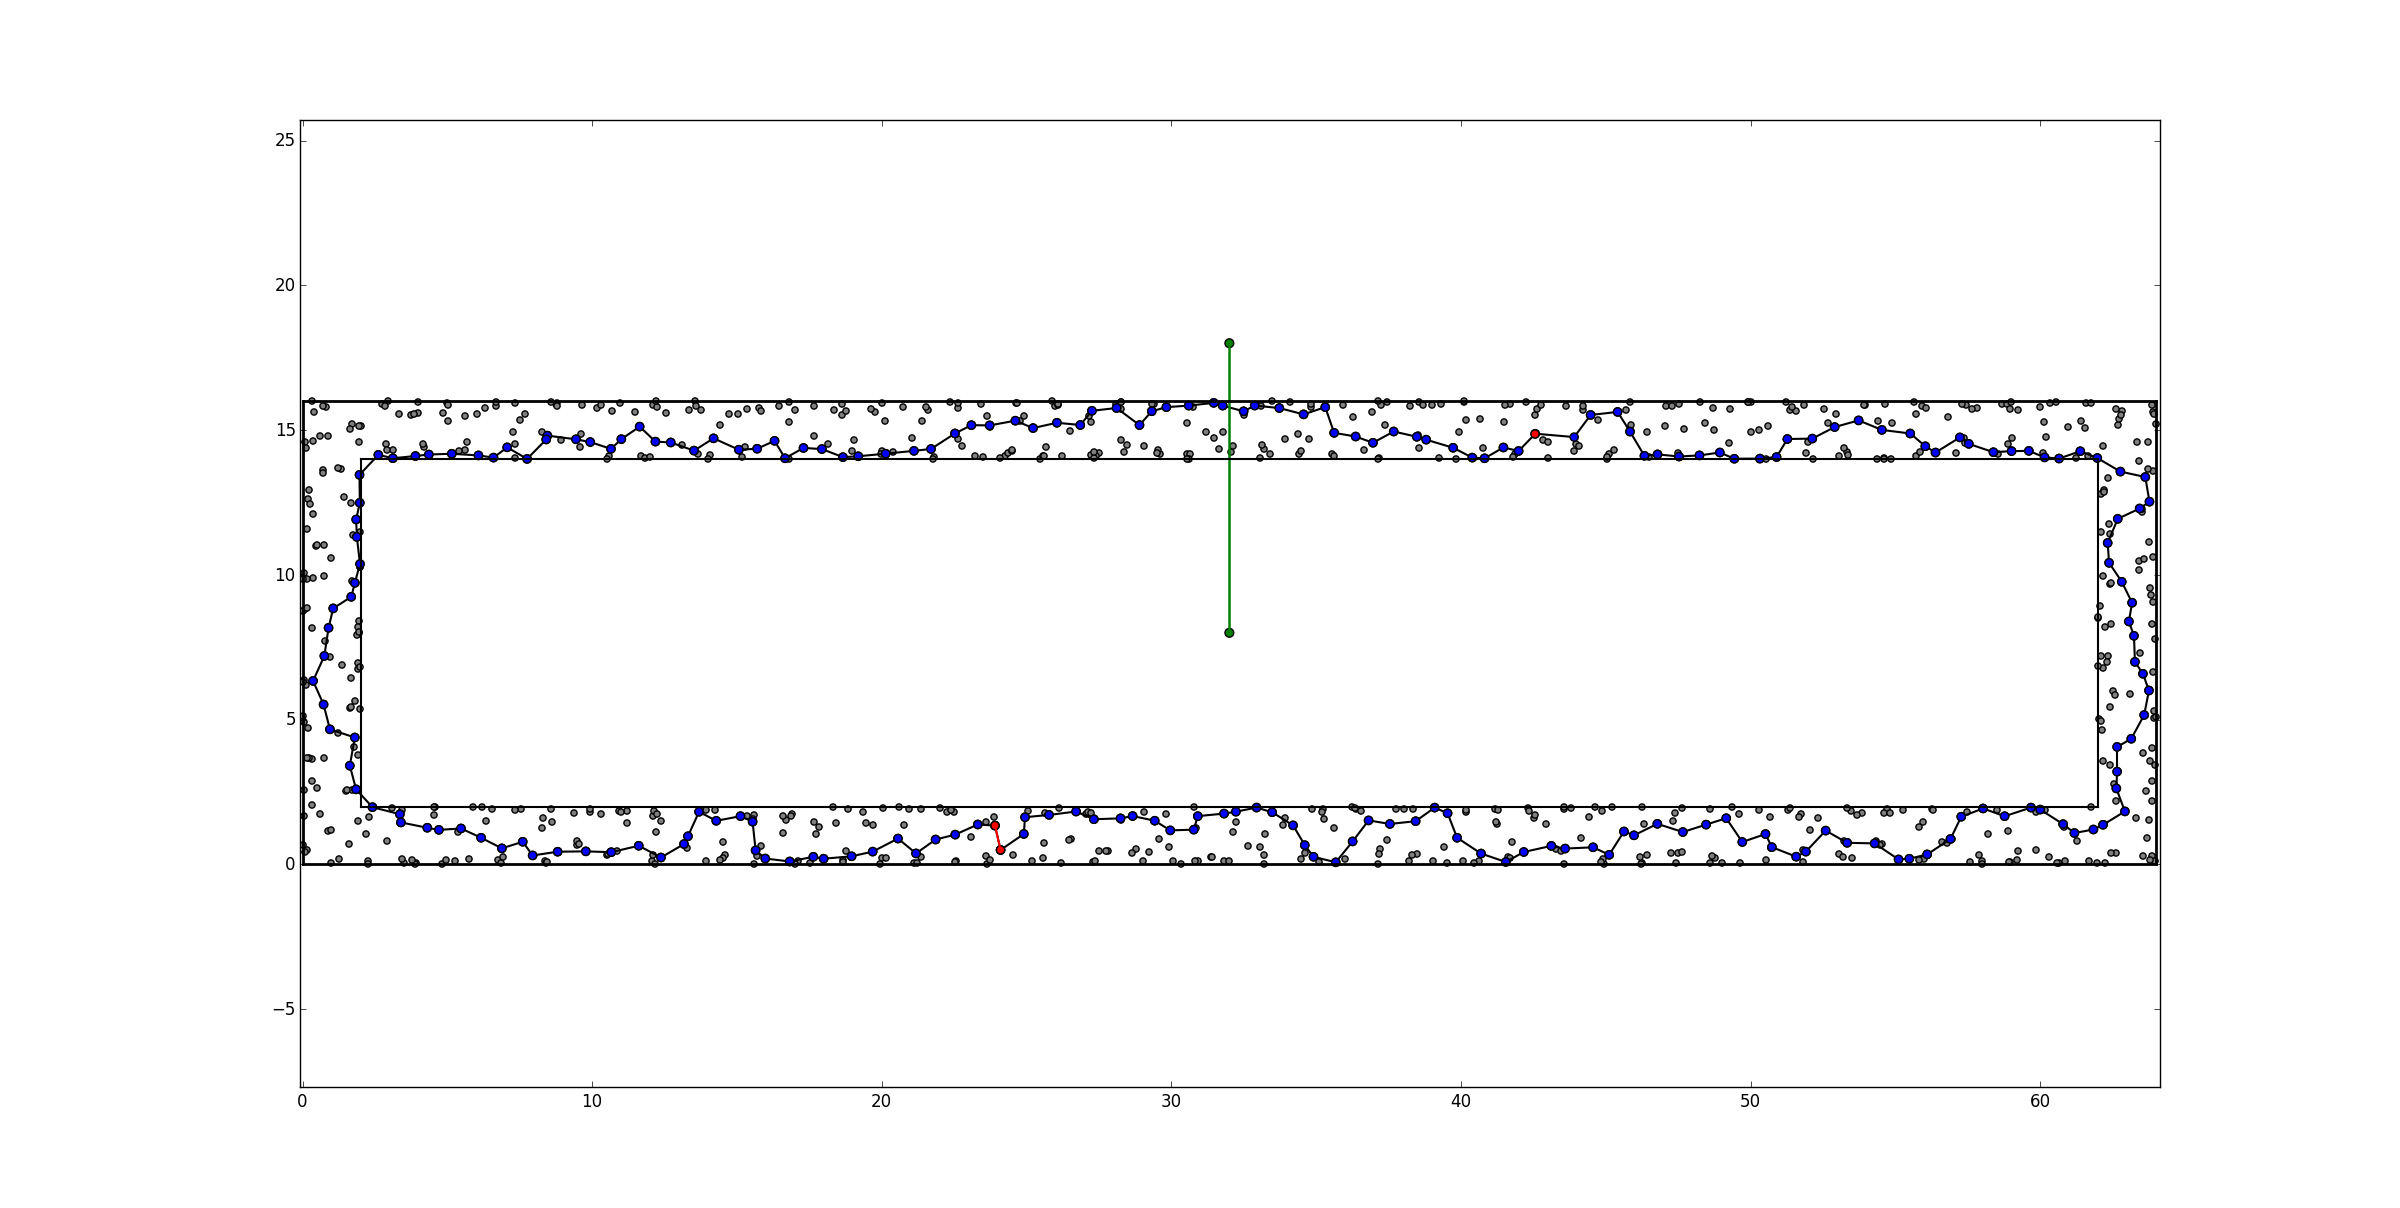
\includegraphics[scale=0.3]{pics/separation-64-1-1000-narrow-2.png}}
\caption{. }
\label{sep-64-1-1000-narrow}
\end{figure}

\begin{figure}
\centerline{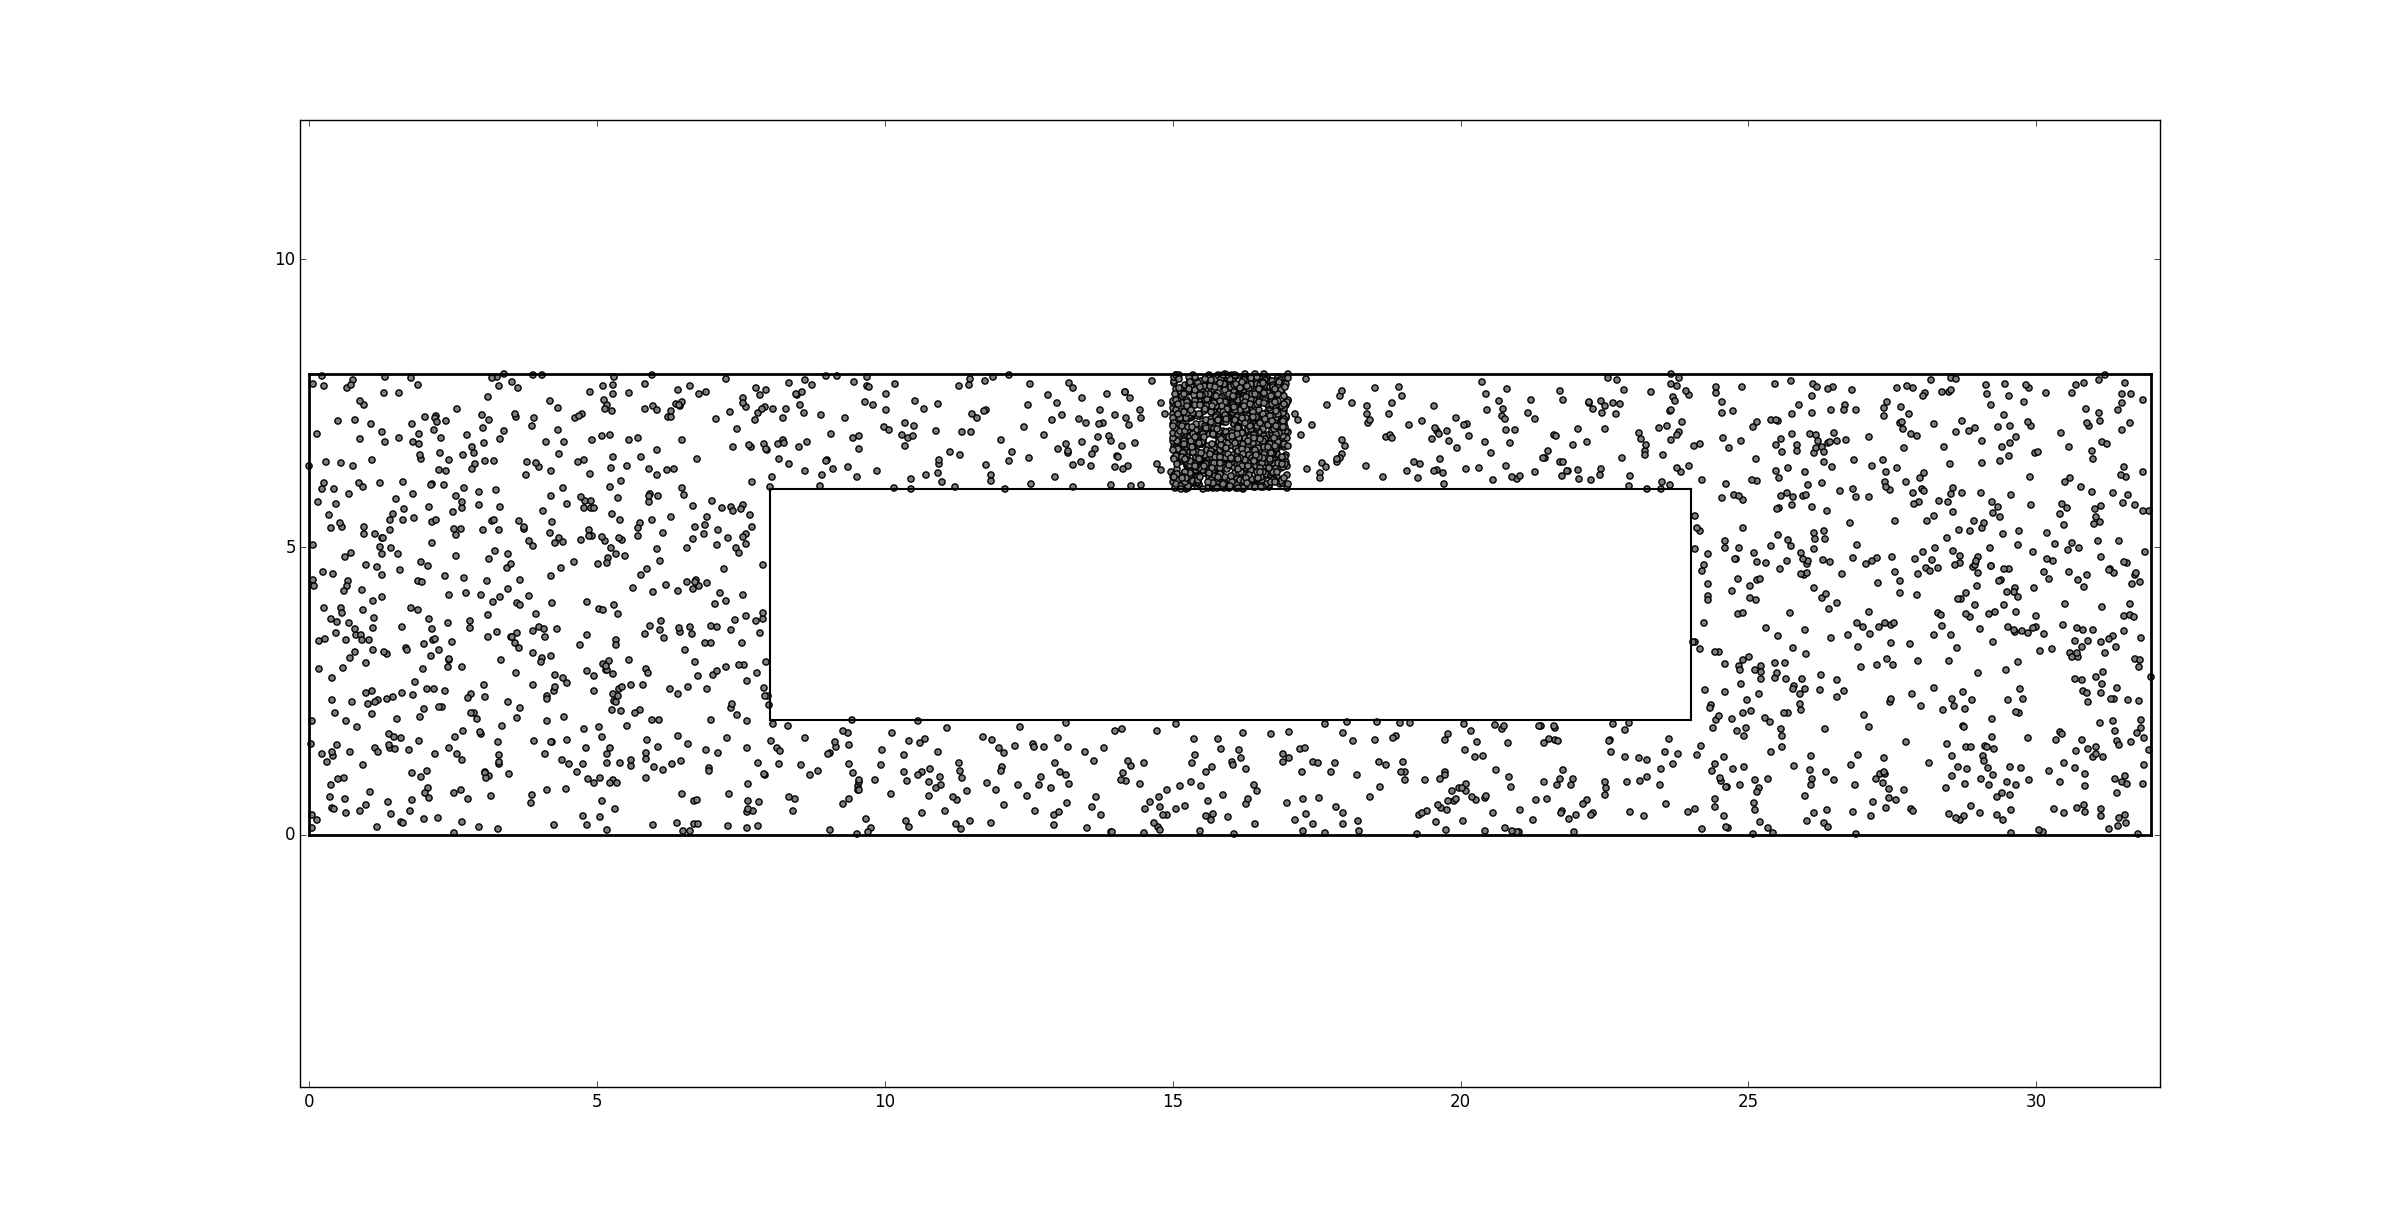
\includegraphics[scale=0.3]{pics/32-1-5000-stuffed.png}}
\caption{. }
\label{sep-stuffed}
\end{figure}

\chapter{Sklepne ugotovitve}
\label{ch4}

\addcontentsline{toc}{chapter}{Literatura}
\begin{thebibliography}{99}
\bibitem{cgalVor}CGAL 4.6 - 2D Voronoi Diagram Adaptor: User Manual. Dostopno na:\\ http://doc.cgal.org/latest/Voronoi\texttt{\_}diagram\texttt{\_}2/index.html
\bibitem{hal}Jean-Daniel Boissonnat, Olivier Devillers, Sylvain Pion, Monique Teillaud, Mariette Yvinec.
Triangulations in CGAL. Computational Geometry, Elsevier, 2002, 22, pp.5-19. $<$inria-00167199$>$.

\end{thebibliography}
\end{document}
